% Copyright Ben Paul Wise. All Rights Reserved.
% Circling Dragons, map and rules for the prototype, version 4: the design memorandum (circling_dragons_map_and_rules_V3.tex,
% v3.3) and the HexKrieg proposal for movement, combat and supply (circling_dragons_hexkrieg_rules.tex, v4.3) combined
% and restructured in the order of the rulebook outline (hexgames/doc/wargame-rulebook-outline.md).  The section
% numbers are the part numbers of the outline: section 3 is the map, section 6 movement, and so on.  The packages and
% page style are shared with the other Circling Dragons documents through sections/cd-style.tex.
\documentclass[11pt]{article}
% Copyright Ben Paul Wise. All Rights Reserved.
% The packages and page style shared by the Circling Dragons documents (circling_dragons_map_and_rules_V3.tex and
% circling_dragons_hexkrieg_rules.tex), taken from the memorandum's preamble on 7 October 2026.  Each document
% gives its own \myversion (the draft version in the footer) and its own pdftitle through \hypersetup.
\usepackage[letterpaper,margin=.85in]{geometry}
\usepackage[T1]{fontenc}\usepackage{lmodern}\usepackage{microtype}
\usepackage{booktabs,longtable,enumitem,amsmath,graphicx}
\usepackage[bookmarksnumbered,bookmarksopen]{hyperref}\usepackage{url}
\usepackage{tikz}


\usepackage{fancyhdr}
\pagestyle{fancy}
\usepackage{lastpage}


\usepackage{xcolor}
\definecolor{darkred}{rgb}{0.55,0,0}
% link and heading colors, from CPVI/shared-tex/prolog-article.tex
\definecolor{myTeal}{RGB}{0, 128, 128}
\definecolor{myBlue1}{RGB}{75, 99, 175}
\hypersetup{
    colorlinks=true,
    linkcolor=myBlue1,
    filecolor=magenta,
    urlcolor=cyan,
    citecolor=myTeal
}
\usepackage{sectsty}
\sectionfont{\color{myBlue1}}
\subsectionfont{\color{myBlue1}}
\subsubsectionfont{\color{myBlue1}}


%\rhead{Basic VI-NCP} % default is section
%\lhead{B. P. Wise} % default is subsection

\providecommand{\myversion}{}
\lfoot{\color{darkred}\bf{DRAFT \myversion}}
\cfoot{{\thepage} of {\pageref*{LastPage}}} % asterix suppressed hyperlink
%\rfoot{\today}
\rfoot{\copyright \  Ben P. Wise}

\setlist{nosep}
% Copyright Ben Paul Wise. All Rights Reserved.

\usepackage{array}
% file names in \path may break at underscores and hyphens as well as at slashes
\expandafter\def\expandafter\UrlBreaks\expandafter{\UrlBreaks\do\_\do\-}
% a rule under play test: its number in the list "To the play testers", linked to that list
\newcommand{\ptest}[1]{\hyperlink{ptest}{\textcolor{darkred}{[P#1]}}}
% a full-page illustration drawn by map_graphics/xml/tools/cd/illustrate.py
\newcommand{\illus}[2]{\begin{figure}[p]\centering\includegraphics[width=\textwidth,height=.9\textheight,keepaspectratio]{illustrations/#1.png}\caption{#2}\label{fig:#1}\end{figure}}
\hypersetup{pdftitle={Circling Dragons: Map and Rules for the Prototype}}

% Changes to the major version number are driven only by major restructuring.
% Almost all edits should increment only the minor version number.
\def\myversion{v4.4}

% Copyright Ben Paul Wise. All Rights Reserved.
% The full-page locator map before each section of figures: the standard sheet with the area of the section's
% figures boxed in black.  Shared by circling_dragons_map_and_rules_V3.tex and maneuver_studies_75km.tex; needs
% graphicx and tikz.  The boxes are generated by map_graphics/xml/tools/cd/illustrate.py (locator-boxes.tex).
% The map is set once in a box, so the PDF carries one copy of the image however many locators there are.
% Copyright Ben Paul Wise. All Rights Reserved.
% Generated by map_graphics/xml/tools/cd/illustrate.py; do not edit.  The area each section's figures show
% on the standard sheet, as a TikZ rectangle in fractions of the sheet (x from the left, y from the bottom).
\def\cdboxIchigo{(0.1568,0.0943) rectangle (0.5986,0.6013)}   % 1-ichigo-setup
\def\cdboxReflux{(0.1568,0.0943) rectangle (0.5986,0.6013)}   % 2-reflux-setup
\def\cdboxAugust{(0.3402,0.5942) rectangle (0.9654,0.9891)}   % 3-august-setup
\def\cdboxRace{(0.2587,0.4484) rectangle (0.8432,0.9241)}   % 4-race-setup
\def\cdboxChangsha{(0.3198,0.2297) rectangle (0.4968,0.3746)}   % a1-changsha-position
\def\cdboxHengyang{(0.2995,0.1568) rectangle (0.4764,0.3225)}   % b1-hengyang-position
% Copyright Ben Paul Wise. All Rights Reserved.

\newsavebox{\cdmapbox}
\AtBeginDocument{\sbox{\cdmapbox}{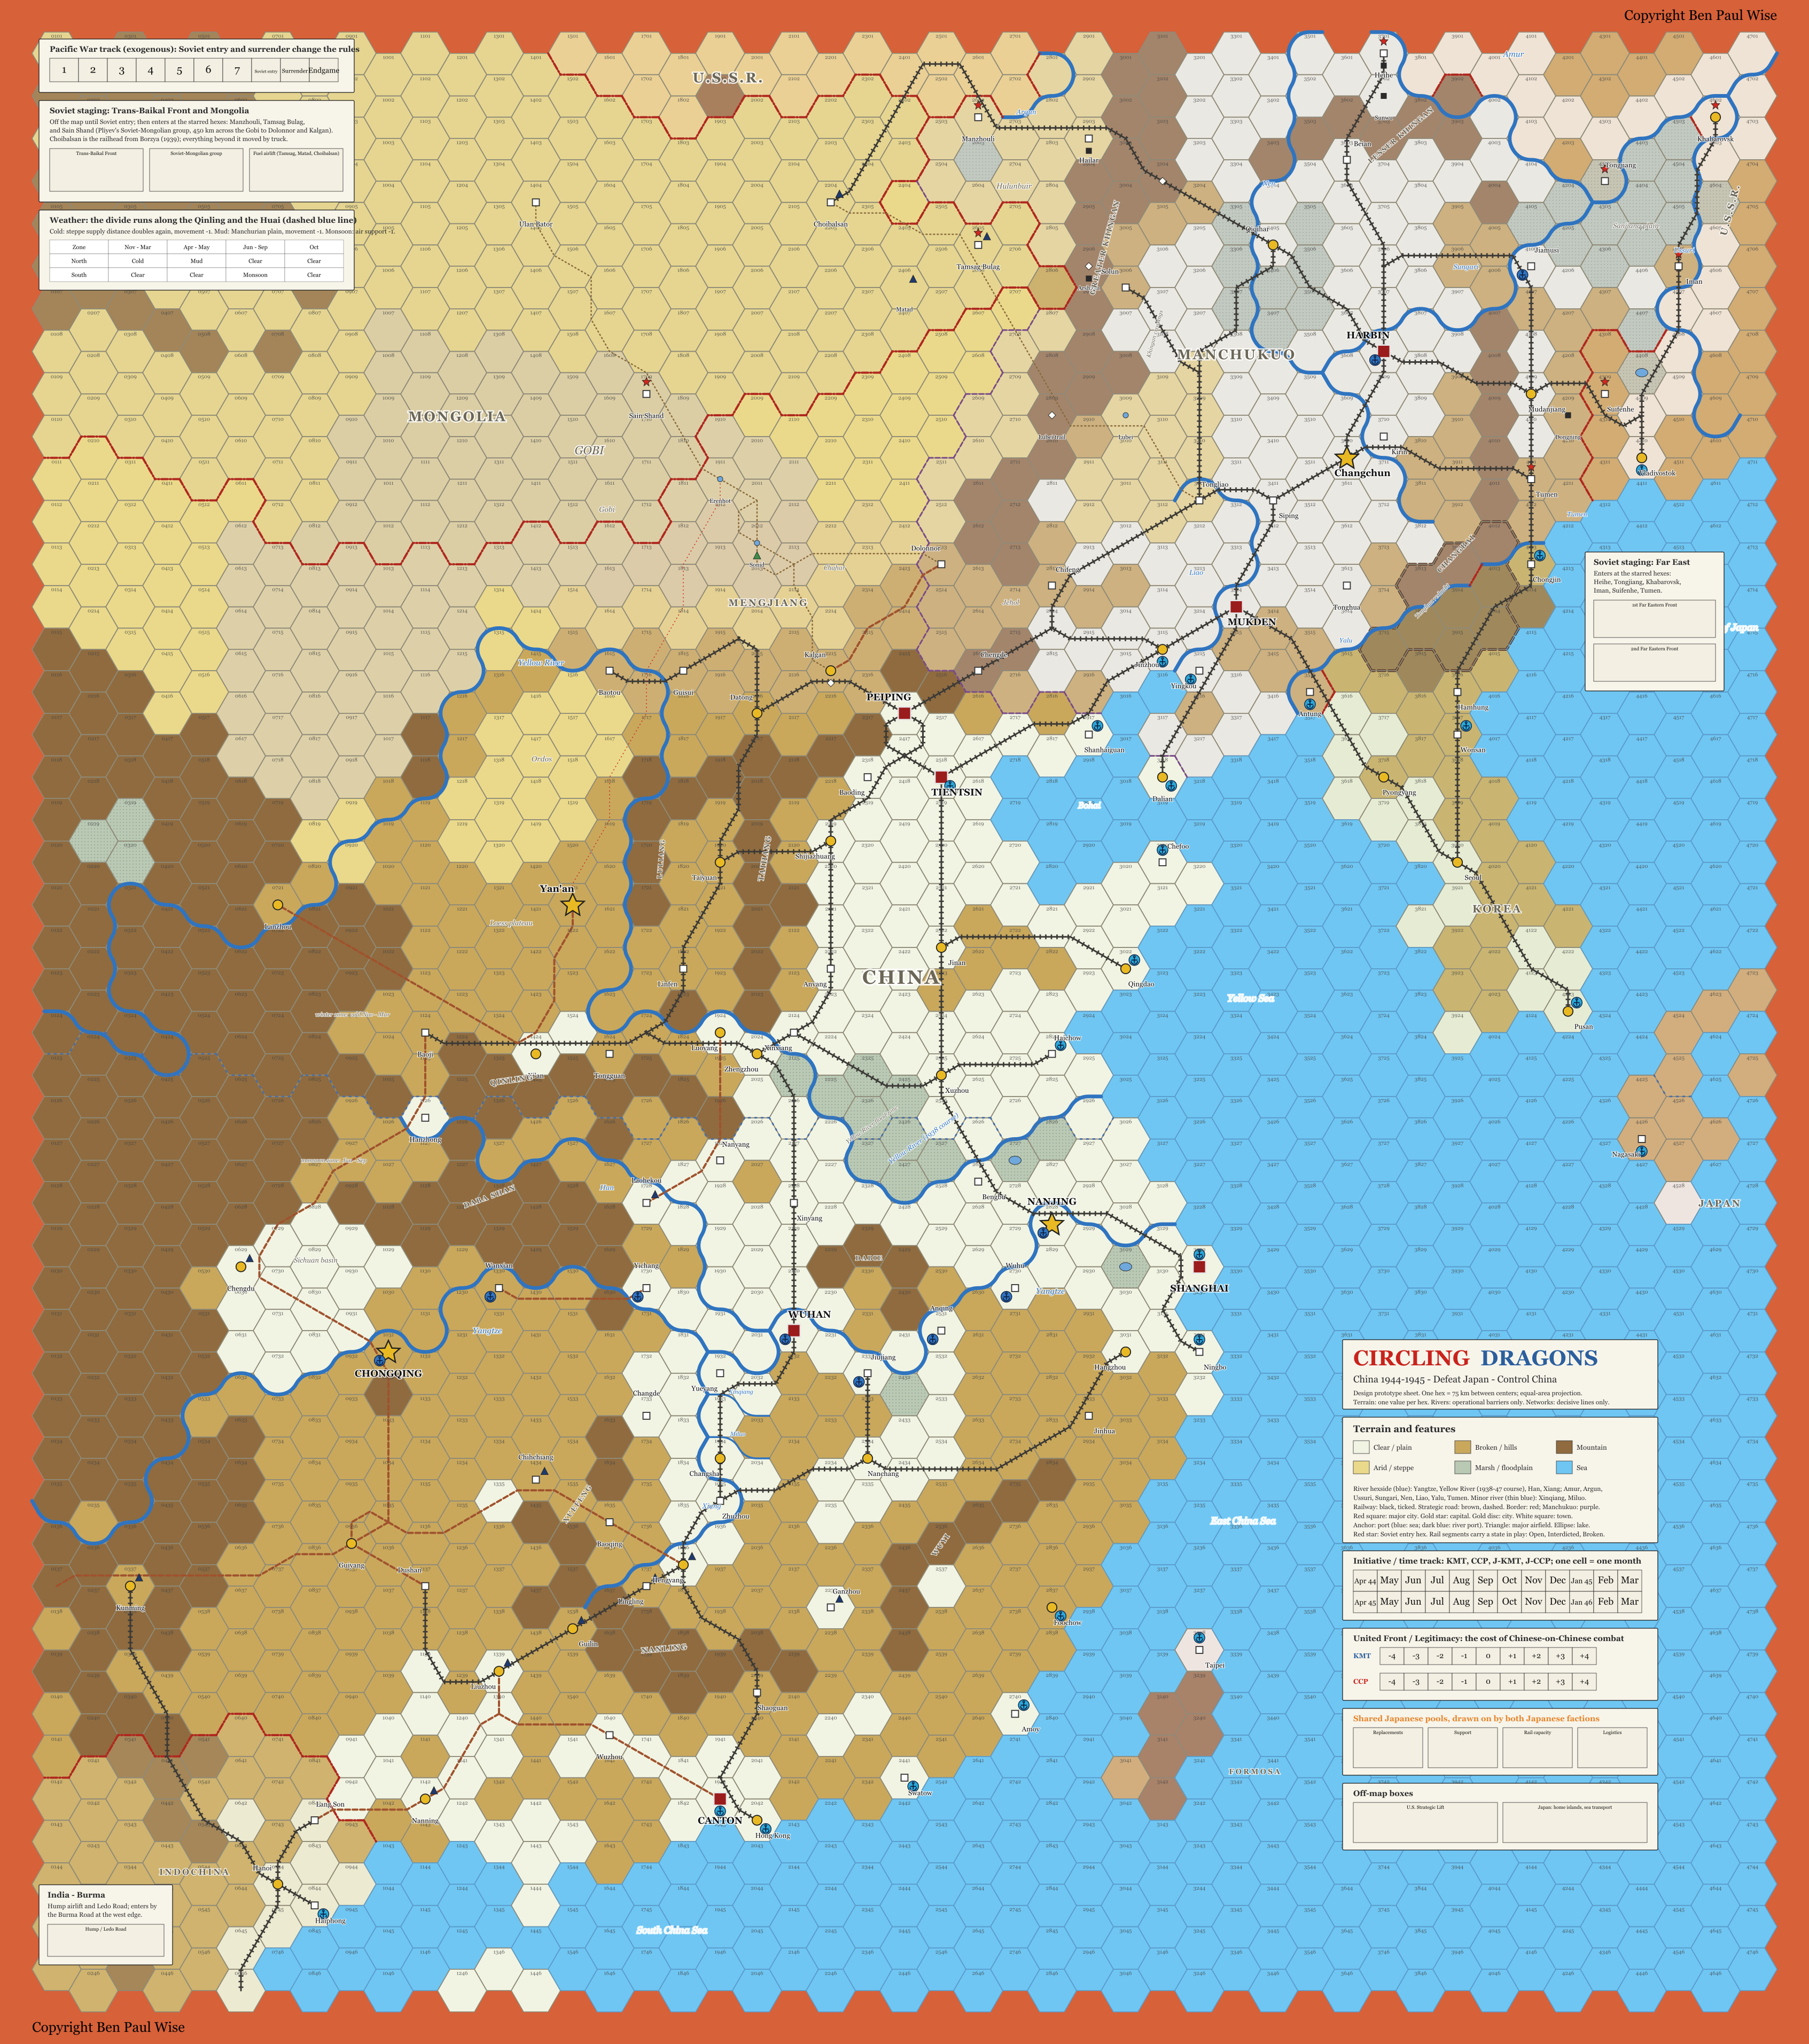
\includegraphics[width=\textwidth,height=.84\textheight,keepaspectratio]{../map_graphics/xml/circling-dragons.png}}}
\newcommand{\locator}[2]{%
  \clearpage
  \begin{figure}[p]\centering
  \begin{tikzpicture}
    \node[anchor=south west,inner sep=0] (map) at (0,0) {\usebox{\cdmapbox}};
    \begin{scope}[x={(map.south east)},y={(map.north west)}]
      \draw[white,line width=5pt] #1;
      \draw[black,line width=2.6pt] #1;
    \end{scope}
  \end{tikzpicture}
  \caption{#2}
  \end{figure}
  \clearpage}
% Copyright Ben Paul Wise. All Rights Reserved.

\title{\textbf{Circling Dragons}\\\large Map and Rules for the Prototype\\\normalsize China, 1944--1946}
\author{}
\date{\textbf{\textcolor{darkred}{DRAFT \myversion}} \today}
\begin{document}
\begin{titlepage}
\centering
\vspace*{\fill}

\includegraphics[width=.92\textwidth]{circling-dragons-logo-V2.pdf}
\vspace*{\fill}
\end{titlepage}
\maketitle
\begin{abstract}
\emph{Circling Dragons} is a two-player strategic-operational game about the defeat of Japan in China, while the KMT and the CCP position themselves for the renewed Chinese Civil War. Each player commands one Chinese faction and the Japanese forces principally opposing the other, the crossed control of \emph{Battle for Germany} and \emph{Downfall}. This version combines two earlier documents, the design memorandum (version 3.3) and the proposal for movement, combat and supply on the HexKrieg model (version 4.3), and arranges their content in the order of a rulebook: introduction, components, map, pieces, sequence of play, movement, combat, supply, the other systems, victory, scenarios, designer's notes and examples. The order follows an outline drawn from seven published rulebooks (\path{hexgames/doc/wargame-rulebook-outline.md}). The rules themselves are those of the two earlier documents; where they differed, the later proposal governs, as section ``How to read these rules'' explains. Every number in the rules is a placeholder for the prototype, and the choices that play testing is to decide are listed, with their alternatives, before the first section. Appendix A, marked as draft, proposes the rules that the earlier documents named but did not write: the time cost of orders, rail capacity and rail state, political actions, air basing, control transfer, headquarters, the junk crossing, Legitimacy, the victory weights and the scenarios.

{\bfseries\footnotesize\color{darkred}This is an AI-generated experimental text, not to be
distributed without written permission.}
\end{abstract}
\clearpage
\begingroup\small\tableofcontents\endgroup
\clearpage

% ======================================================================================================================
% Part 0 of the outline: front matter
% ======================================================================================================================
\section*{How to read these rules}
\phantomsection\addcontentsline{toc}{section}{How to read these rules}\label{sec:howto}
\markboth{HOW TO READ THESE RULES}{HOW TO READ THESE RULES}
\paragraph{Order.} Sections 1 and 2 introduce the game and its components. Sections 3 to 8 give the map, the pieces, the sequence of play, and the rules of movement, combat and supply; each of the last three is divided into land, sea and air. Sections 9 to 14 give the other systems: command, reinforcements and recovery, weather, hidden information, the special rules, and victory. Section 15 gives the four situations of the prototype, section 16 the provisional rules, section 17 the designer's notes, section 18 the examples of play, section 19 a list of the charts and tables, and section 20 a glossary.

\paragraph{Sources of the rules.} The rules of sections 5 to 8 that govern movement, combat and supply come from the HexKrieg proposal (version 4.3), and the rest from the design memorandum (version 3.3). Where the two differed, the proposal governs, because it was written to replace the memorandum's provisional rules. The differences are four: zones of control now stop movement as well as supply; each piece has an offense and a defense in place of one strength; supply is graded in four levels and carried by supply pieces; and a formation out of supply is at level 0 rather than simply out of supply. The two maneuver studies of section \ref{sec:maneuvers} were drawn under the memorandum's provisional rules, which they list as R1 to R7 (section \ref{sub:mrules}); section \ref{sub:checks} shows what the present rules give for the same events.

\paragraph{Terms.} \emph{Must} states a requirement and \emph{may} a permission. \emph{A piece} means any one piece, and \emph{one piece} exactly one. A \emph{unit piece} is a combat formation; a \emph{marker} records information and has no strength. Terms defined in the rules are in bold where they are defined and are collected in the glossary, section \ref{sec:glossary}.

\paragraph{Draft rules.} Appendix \ref{app:draft} drafts the rules that the sections name but do not yet write. It is marked as draft throughout and is not part of the rules; each place in the rules that lacks a rule points to its draft.

\paragraph{Marks.} A number in dark red brackets, e.g., \ptest{1}, marks a choice under play test and links to the list that follows. Paragraphs labeled \emph{Example} illustrate a rule and add nothing to it. Hexes are named by four-digit numbers, e.g., 2034, as on the map.

\paragraph{Play testing.} Play testing is meant to show whether these rules enable the operations of 1944 and 1945 to be reproduced for the right reasons and at the right pace, and whether the decisions they pose have more than one reasonable answer. Interesting yet plausible variations should be possible; changes to enhance those variations are welcome. Observations of every kind are useful, especially where a rule gave a result that seems historically wrong, where a choice was obvious, or where a rule was hard to apply.
\clearpage

\section*{To the play testers}
\phantomsection\addcontentsline{toc}{section}{To the play testers}\hypertarget{ptest}{}\label{sec:playtest}
\markboth{TO THE PLAY TESTERS}{TO THE PLAY TESTERS}
These rules are a first version for the prototype, and they will change. Most of their numbers are placeholders, and many of the rules are choices between alternatives that only play testing can settle. Table \ref{tab:choices} lists those choices with the alternatives considered so far, and in the rules each choice is marked with its number, e.g., \ptest{1}. Reports on any of them, and suggestions for other changes, are welcome.

{\footnotesize
\begin{longtable}{@{}>{\raggedright\arraybackslash}p{.05\textwidth}>{\raggedright\arraybackslash}p{.50\textwidth}>{\raggedright\arraybackslash}p{.38\textwidth}@{}}
\caption{Choices under play test}\label{tab:choices}\\
\toprule
No. & The rule now & Alternatives \\
\midrule
\endfirsthead
\toprule
No. & The rule now & Alternatives \\
\midrule
\endhead
\bottomrule
\endfoot
\multicolumn{3}{@{}l}{\textbf{Supply} (section \ref{sub:supply})} \\
P1 & Supply pieces carry supply, with a reach $R$ counted along the network; $R$ starts at 6 network hexes. & A longer or a shorter reach. With a reach longer than any distance on the sheet, the rule becomes a plain trace along the network. \\
P2 & Each relay through a supply piece costs one level. & No loss per relay, so that only the reach and the number of pieces matter. \\
P3 & Supply pieces: Japanese 6 in China and 2 in Manchuria and Korea, KMT 5. & Other counts, e.g., one per front or one per war area. \\
P4 & The CCP has no supply pieces; its base areas are its sources. & CCP supply pieces, or presence markers that relay supply. \\
P5 & Japanese supply pieces belong to a front and are moved by its controller. & Drawn from the shared Japanese logistics pool, so that both Japanese controllers compete for them. \\
P6 & The Soviet groupings keep the Mongolian rules, with the roll of the fuel airlift. & Soviet forward depots as supply pieces moving along the tracks. \\
P7 & Local paths costing 3, 5 and 7 points allow levels 3, 2 and 1; the multipliers of table \ref{tab:supply}; formations on foot keep their whole allowance at every level. & Other thresholds; the multipliers of the HexKrieg draft, which also slow formations on foot. \\
\multicolumn{3}{@{}l}{\textbf{Combat} (section \ref{sub:combat})} \\
P8 & Assault losses: a piece that attacks a fortified city or a Kwantung fortified zone without taking it loses one step on a roll of 8 to 10. & Fortified cities only; another rate. \\
P9 & The combat table is the HexKrieg table moved one row toward the defender, and the odds are rounded in the defender's favor (table \ref{tab:crt}). & The HexKrieg table and rounding, equations \eqref{eq:hkodds_A} and \eqref{eq:hkodds_B}. \\
P10 & Defense one more than offense for KMT group armies and railway garrisons, one less for the tank formations and the cavalry-mechanized group, equal otherwise (table \ref{tab:pieces}). & Other values. \\
P11 & Air support raises its side's fire in one combat per activation, within four hexes, by half. & Air supply only, without a combat effect; another range or effect. \\
P12 & Fire across a major river is halved. & No effect of rivers on combat, so that they act on movement and supply only. \\
P13 & A defender may withdraw before combat when it is attacked as well as when an enemy moves adjacent, at a cost of one initiative space. & The trigger of R3 alone; another cost. \\
\multicolumn{3}{@{}l}{\textbf{Movement} (sections \ref{sub:terrain} and \ref{sub:move})} \\
P14 & Entering an enemy zone of control ends a move. & Zones that only cut supply, as in R1; four moves of the figures then need no extra activation. \\
P15 & Movement costs: clear and broken 1, mountain and marsh 2, a minor river 1 extra, a major river 2 extra, and 0.5 per edge along a line (table \ref{tab:terrain}). & Broken at 2, under which four moves of the figures exceed their allowances; other river costs. \\
P16 & KMT and CCP pieces exert no zones of control on each other before the surrender. & Zones between them at all times, or from the first Chinese-on-Chinese attack in the area. \\
\end{longtable}
}
The provisional rules of the political layer (section \ref{sub:political}) are also under test; each is to be kept only if play testing shows that it improves the game.
\clearpage

% ======================================================================================================================
% Part 1: introduction
% ======================================================================================================================
\section{Introduction}\label{sec:intro}
\subsection{What the game is about}
\emph{Circling Dragons} covers the last two years of the war in China, from the spring of 1944 to the spring of 1946. Two Chinese parties fought Japan in those years: the Nationalist government of Chiang Kai-shek, the KMT (Kuomintang), and the Chinese Communist Party of Mao Zedong, the CCP. They were allies in name, in a united front against Japan, and each expected to fight the other once Japan was beaten. The game is about that double contest. Each Chinese faction must help to defeat Japan, but each must also come out of the war stronger than its rival. The defeat of Japan is therefore a shared aim, and the winner is the faction better placed when the war against Japan has turned into the civil war.

The situation is historical. The game is designed so that the players can reproduce the historical battles with reasonable fidelity and can also explore interesting and plausible variations (section \ref{sub:variations}).

\subsection{Scale}
\begin{itemize}
\item \textbf{Map:} 75 km between the centers of neighboring hexes, on a sheet of 47 by 46 hexes covering China, Manchuria, Korea and Mongolia.
\item \textbf{Time:} no fixed turns. Each faction acts when its marker on the time track is furthest behind, and a calendar interval is about one month (section \ref{sec:sequence}).
\item \textbf{Pieces:} Japanese divisions, KMT group armies and armies, CCP field forces, Soviet armies and puppet armies, of one to four steps; about 105 formations on the map at the start (section \ref{sec:pieces}).
\item \textbf{Players:} two, the KMT player and the CCP player. The design is meant for AI agents as well as for human players.
\item \textbf{Dice:} one ten-sided die.
\end{itemize}

\subsection{Two players, four factions}\label{sub:intro-control}
Neither player is Japan. Each commands one Chinese faction and, in addition, the Japanese forces that principally face the other Chinese faction (table \ref{tab:intro-control}). This arrangement, called crossed control, is taken from the games \emph{Battle for Germany} and \emph{Downfall}.

\begin{table}[ht]
\centering\small
\begin{tabular}{@{}lll@{}}
\toprule
Player & Own faction & Japanese forces commanded \\
\midrule
KMT player & the KMT armies & those facing the CCP, chiefly the garrisons of North China \\
CCP player & the CCP field forces and base areas & those facing the KMT, chiefly the armies of Ichi-Go \\
\bottomrule
\end{tabular}
\caption{Who commands what}\label{tab:intro-control}
\end{table}

The CCP player therefore conducts Ichi-Go against the KMT, and the KMT player uses the Japanese garrisons of North China against the CCP's base areas. Each player gains when the Japanese forces under that player's command damage the rival faction, but three things limit that use. First, each Japanese operation must serve the Japanese strategic directive in force, e.g., opening the railway corridor or holding the railways; the player chooses only how. Second, both Japanese commands draw on shared pools of operational support, replacements, rail capacity and logistics, so what one player spends with Japanese forces is lost to the Japanese forces of the other. Third, a Japanese formation changes controller when it moves from one front to the other, as many did in 1945. The two Chinese factions may also fight each other directly, but each such battle costs standing on a Legitimacy track, which measures political standing and foreign support; for most of the game each player therefore prefers that Japanese forces do the damage.

Two outside powers take part without a player of their own. The United States supplies air support, a limited Strategic Lift that moves KMT armies by air and sea, and Marines who hold ports after the surrender. The Soviet groupings that enter Manchuria in August 1945 follow a script: they move along fixed axes, and the players influence only the few choices the script leaves open.

\subsection{The four operations and the historical course}\label{sub:course}
Four large operations mark the period. Section \ref{sec:scenarios} gives the frame, the pieces and the rules of each.
\begin{itemize}
\item \textbf{Ichi-Go}, April to December 1944: the largest Japanese offensive of the war in China, which opened a railway corridor to Indochina and took the American air bases in south China.
\item \textbf{The reflux of 1945}, January to August: the Japanese withdrew from the south toward the north and the coast, and both Chinese factions moved into the ground they left.
\item \textbf{August 1945}: the Soviet Union entered the war and occupied Manchuria, and Japan surrendered.
\item \textbf{The race}, from September 1945: the KMT and the CCP raced each other for the cities, railways, ports and arms dumps of North China and Manchuria.
\end{itemize}

A game follows the course of the war. In 1944 the CCP player's Japanese forces conduct Ichi-Go against the KMT, while the KMT player's Japanese garrisons attack the CCP's bases in the north and the CCP extends its presence behind them. In 1945 the Japanese withdraw toward the north and the coast; formations change controller as they change front, and both Chinese factions move into the ground the Japanese leave. In August the Soviets enter Manchuria, and the KMT player decides whether to accept the Sino-Soviet treaty, which costs Legitimacy but secures Soviet recognition of the Nationalist government. Japan's surrender changes the rules. Japanese offensives end, and Japanese garrisons hold their cities until a Chinese faction takes them over. The two Chinese factions then race for what Japan leaves, the KMT with American air and sea lift, the CCP on foot and by junk across the Bohai, while the Soviets withdraw from Manchuria in stages.

\subsection{Variations}\label{sub:variations}
The rules leave these decisions open, and each can take the game away from the historical course.
\begin{itemize}
\item \textbf{The conduct of the Japanese offensives.} A directive names the objective; the controlling player chooses where to attack, which formations to destroy rather than push aside, and how much of the shared pools to spend.
\item \textbf{Chinese-on-Chinese fighting.} Either player may attack the rival faction directly at a Legitimacy cost (section \ref{sub:civil}).
\item \textbf{The Sino-Soviet treaty.} The KMT player may accept or refuse it; each answer has a cost (section \ref{sub:treaty}).
\item \textbf{The Tonghua redoubt.} The Kwantung Army may withdraw into it at Soviet entry, which the historical Kwantung Army planned and did not do (section \ref{sub:political}).
\item \textbf{The race.} Where the KMT spends Strategic Lift, and where the CCP sends its field forces, columns and presence.
\item \textbf{The Soviet directive.} Which objective comes first, and when a halted grouping resumes.
\end{itemize}

\subsection{Design features and their purposes}\label{sub:design}
\begin{enumerate}
\item \textbf{Two players, four factions.} The game builds on the system of \emph{Downfall} to represent Mao Zedong and Chiang Kai-shek cooperating to defeat the Japanese while each positions his faction for the coming civil war.
\item \textbf{Historical fidelity with room for variation.} The game should make it possible to replay the historical battles with reasonable fidelity while enabling interesting and plausible variations.
\item \textbf{75 km per hex.} The first sheet used 100 km, close to \emph{Downfall}'s 110 km land hexes; at that scale the Hunan corridor was too narrow for the defender's maneuver (section \ref{sec:maneuvers}).
\item \textbf{Operational focus.} The game does not force players into excessive tactical detail. Railways, major river crossings, strategic roads, ports, airfields and mountain corridors matter more than fine terrain differentiation, and the map is a sparse transport network laid over coarse terrain barriers.
\item \textbf{A continuous time track.} The initiative system is similar to that of \emph{Downfall}; a full calendar interval is about one month. A small action brings a faction back into play soon; a large operation leaves it waiting while the others act.
\item \textbf{Two kinds of control.} KMT and Japanese power is primarily conventional control of nodes and communications. Much CCP power is rural presence and base control, capable of interdiction and political expansion.
\item \textbf{Manchuria.} The map gives Manchuria enough space for the Soviet western, eastern and northeastern approaches.
\item \textbf{The surrender as a change of phase.} The August 1945 surrender changes the phase of the game: Japanese combat power declines, and railways, ports, cities, surrender sites and access to Manchuria become the principal objectives.
\item \textbf{Movement, combat and supply on the HexKrieg model.} These three subjects are taken from HexKrieg, a hex game built as a testbed for artificial-intelligence agents, and changed only where \emph{Circling Dragons} requires it (section \ref{sub:hexkrieg}). Supply is carried by supply pieces along the transport network, so that a deep advance such as Ichi-Go must pause while its supply catches up.
\end{enumerate}

\subsection{The game in outline}\label{sub:outline}
This subsection gives a first picture of how the game is played. It contains no rules of its own; the later sections govern.

\paragraph{Time and initiative.} There are no game turns in the usual sense. Each of the four factions, i.e., the KMT, the CCP, the Japanese facing the KMT and the Japanese facing the CCP, has a marker on a time track. The faction whose marker is furthest behind acts next. It gives orders, to move, to attack, to move by rail, to refit, to act politically, or to cut or repair transport, and each order moves its marker forward by the time the order takes. Dates on the calendar bring the seasons, reinforcements, the Soviet entry and the Japanese surrender. One turn of a faction on the time track is called an activation: the active faction moves its pieces and declares its attacks, the attacks are resolved, and the supply of every piece on the map is checked.

\paragraph{The map.} At 75 km a hex holds a city and the country around it, and a hex can hold two pieces. Each hex has one kind of terrain: clear, broken (hills and rough country), mountain, marsh, steppe, desert or sea. The major rivers, among them the Yangtze, the Yellow River and the rivers of Manchuria, run along the sides of hexes and are hard to cross; two minor rivers north of Changsha are shown because they shaped the battles there. Outer Mongolia is open only to the Soviets, who prepare their August offensive there. The most important features are the railways and the few strategic roads. China in 1944 had few of either, and armies, supplies and offensives followed them. Most objectives lie on the network: junctions, bridges, cities, airfields and ports.

\paragraph{The pieces.} The combat pieces are formations, each with an attack value, a defense value, a movement allowance, and one to four steps. A step is a share of the formation's strength: a formation that loses a step becomes weaker, and one that loses its last step is removed. Other counters record information rather than strength: the CCP's presence markers, which show the party's influence in the countryside and become base areas where it is established; control markers for cities; markers for the state of railways, bridges, ports and airfields; fortified cities; and the Japanese directives and pools. Air-support pieces stand for the air forces, e.g., the US Fourteenth Air Force, and supply pieces carry supply forward along the network.

\paragraph{Movement.} A formation spends movement points as it moves from hex to hex. Open ground is cheap, mountains and marshes cost more, crossing a river costs extra, and movement along a railway or road costs least. Each formation has a zone of control, the hexes around it except across a major river or into mountains; an enemy formation that enters one of those hexes must stop there.

\paragraph{Combat.} The active faction chooses which enemy hexes to attack, and the defenders fire back, so an attack can cost the attacker as well. For each defending formation the strength aimed at it is compared with its defense, and one roll of a ten-sided die gives the result: no effect, a retreat, the loss of one step, or the loss of two. Terrain, rivers, fortified cities, attacks from several sides, air support and supply change the strengths. A defender in rough country or behind a river may step back before the attack instead of standing.

\paragraph{Supply.} Supply starts at sources, i.e., ports, capitals, depots, railheads and the CCP's base areas, and runs along the transport network. Supply pieces relay it forward, and each relay delivers a little less. A formation away from the network must find a short path to a supplied hex. The result is one of four supply levels: a poorly supplied formation attacks and defends less well, and a formation that is cut off loses strength if it stays cut off.

\subsection{How the game is won, in brief}
The winner is the player whose faction has the better Postwar Position when the transition to civil war is complete, not the player who did more damage to Japan. Postwar Position counts politically valuable territory, major cities, intact armed strength and Legitimacy, less a deduction for dependence on others and for disrupted communications, and the two factions weigh these differently: the KMT values recognized authority, cities, ports, rail junctions and intact armies; the CCP values connected base areas, popular support, its position in North China, access to Manchuria and intact field forces. Each decision therefore has two sides: its effect on Japan, and its effect on the rival that will still be there when Japan is gone. Section \ref{sec:victory} gives the full rule.

% ======================================================================================================================
% Part 2: components
% ======================================================================================================================
\section{Components}\label{sec:components}
\begin{itemize}
\item \textbf{The map:} the standard sheet, 47 by 46 hexes at 75 km, about 32 by 36 inches with 3/4 inch hexes, printed on two map sheets of 22 by 34 inches joined along their long edges (section \ref{sec:map}).
\item \textbf{The counters:} 263 counters on two sheets of 12 by 12, i.e., 126 unit pieces, 5 air-support pieces, 13 supply pieces and the markers (section \ref{sec:pieces}). The counter set does not yet carry the defense values of table \ref{tab:pieces} or step markers.
\item \textbf{Tracks and displays:} the time track with the four initiative markers and the calendar; the Legitimacy (United Front) track; the Pacific War track, on which the Soviet entry, the Sino-Soviet treaty and the surrender are dated events; the Soviet withdrawal track; and the shared Japanese pools of operational support, replacements, rail capacity and logistics.\item \textbf{A ten-sided die.}
\item \textbf{This document}, with the charts and tables listed in section \ref{sec:charts}.
\end{itemize}

% ======================================================================================================================
% Part 3: the map
% ======================================================================================================================
\section{The map}\label{sec:map}
\subsection{Grid and extent}
The map uses \textbf{75 km per hex} and allows modest distortion where it preserves the topology of junctions and corridors. Its hexes have flat tops and are numbered by column and row in four digits, from 0101. It extends from Mongolia and Soviet territory and Manchuria in the north to Guangxi and northern Indochina in the south, and from the coast west to the Chongqing--Chengdu and Shaanxi rear areas. Remote western China is compressed or handled with off-map boxes, so that the board area goes to the contested corridors. Of the sheet's 2,162 hexes, 1,187 are in play (China proper 895, Manchukuo 247, Korea 45), and 242 Mongolian hexes are open to Soviet formations only.

\subsection{The standard sheet at 75 km}\label{sub:sheet75}
% Copyright Ben Paul Wise. All Rights Reserved.
% The standard sheet at 75 km: shared by circling_dragons_map_and_rules_V3.tex and maneuver_studies_75km.tex,
% each of which gives the heading.  Needs the labels sec:maneuvers and sub:mrules (maneuver-studies.tex).
The standard sheet has 75 km between hex centers. It replaced the first sheet, at 100 km, in October 2026, because at 100 km the Hunan corridor is too narrow for two maneuvers that decided its battles: Xue Yue's defense of Changsha in 1939--42 and the Japanese envelopment of Hengyang in 1944 (section~\ref{sec:maneuvers}).

Both sheets cover the same area and are built by the same programs from the same sources, so the scale is a setting of the build and the first sheet can still be produced for comparison. Every ruling made on the 100 km sheet was carried over: the named mountain ranges, the lakes and the Tonghua redoubt are lists of 100 km hexes, and each 75 km hex whose center falls in a listed hex takes the ruling. Three coastal hexes, each just under half land, were ruled land so that the railways of the Liaodong peninsula, the south shore of Hangzhou Bay and the Korean west coast stay on land. At Yueyang the Yangtze was moved to the north side of the city's hex, so that the railway south to Changsha does not cross it. Between Tongguan and Zhengzhou the Yellow River was moved to the north side of the Sanmenxia and Luoyang hexes, so that the Longhai railway stays on the south bank and crosses the river only on its 1938--47 course east of Zhengzhou. The Ussuri was extended two hexsides to join the Amur at Khabarovsk. The sheet passes the same validation and network checks as the first one.

\begin{center}
\begin{tabular}{lrr}
\toprule & First sheet & Standard sheet \\\midrule
Distance between hex centers & 100 km & 75 km \\
Columns by rows & 35 by 34 & 47 by 46 \\
Hexes on the sheet & 1,190 & 2,162 \\
Hexes in play (China, Manchukuo, Korea) & 672 & 1,187 \\
Mongolian hexes, open to Soviet formations only & 131 & 242 \\
Clear hexes across the corridor at Changsha & 2 & 3 \\
Clear hexes across the corridor at Hengyang & 2 & 3 \\
Hexes from Yueyang to Changsha & 1 & 2 \\
Hexes from Hankow to Dushan along the corridor & 12 & 15 \\
Sheet size with 3/4 inch hexes & 24 by 27 in & 32 by 36 in \\
\bottomrule
\end{tabular}
\end{center}

Of the hexes in play, the two sheets have nearly the same terrain: clear 26 and 27 percent, broken 33 and 32, mountain 24 and 23, steppe 15 and 15, marsh 3 and 3. The smaller hex does not make the country look flatter, so the terrain thresholds were left unchanged.

The standard sheet adds one line class, the \textbf{minor river}, drawn thinner than the major rivers and printed only where a minor river shaped a campaign. Two are printed: the Xinqiang and the Miluo, the delay lines north of Changsha on which Xue Yue's screens stood. Each crosses the railway column and the lane east of it, and each runs into the Xiang. The Laodao, the third of his lines, lies inside the Changsha hex and is not printed. In the provisional rules a minor river costs less to cross than a major river, and a formation behind one may withdraw before combat (section~\ref{sub:mrules}).

At 3/4 inch hexes the sheet is about 32 by 36 inches and fits on two 22 by 34 inch map sheets joined along their long edges. To keep the density of pieces of the first estimate, the counter set was grown to 126 unit pieces and 250 counters in all.

\begin{figure}[p]\centering
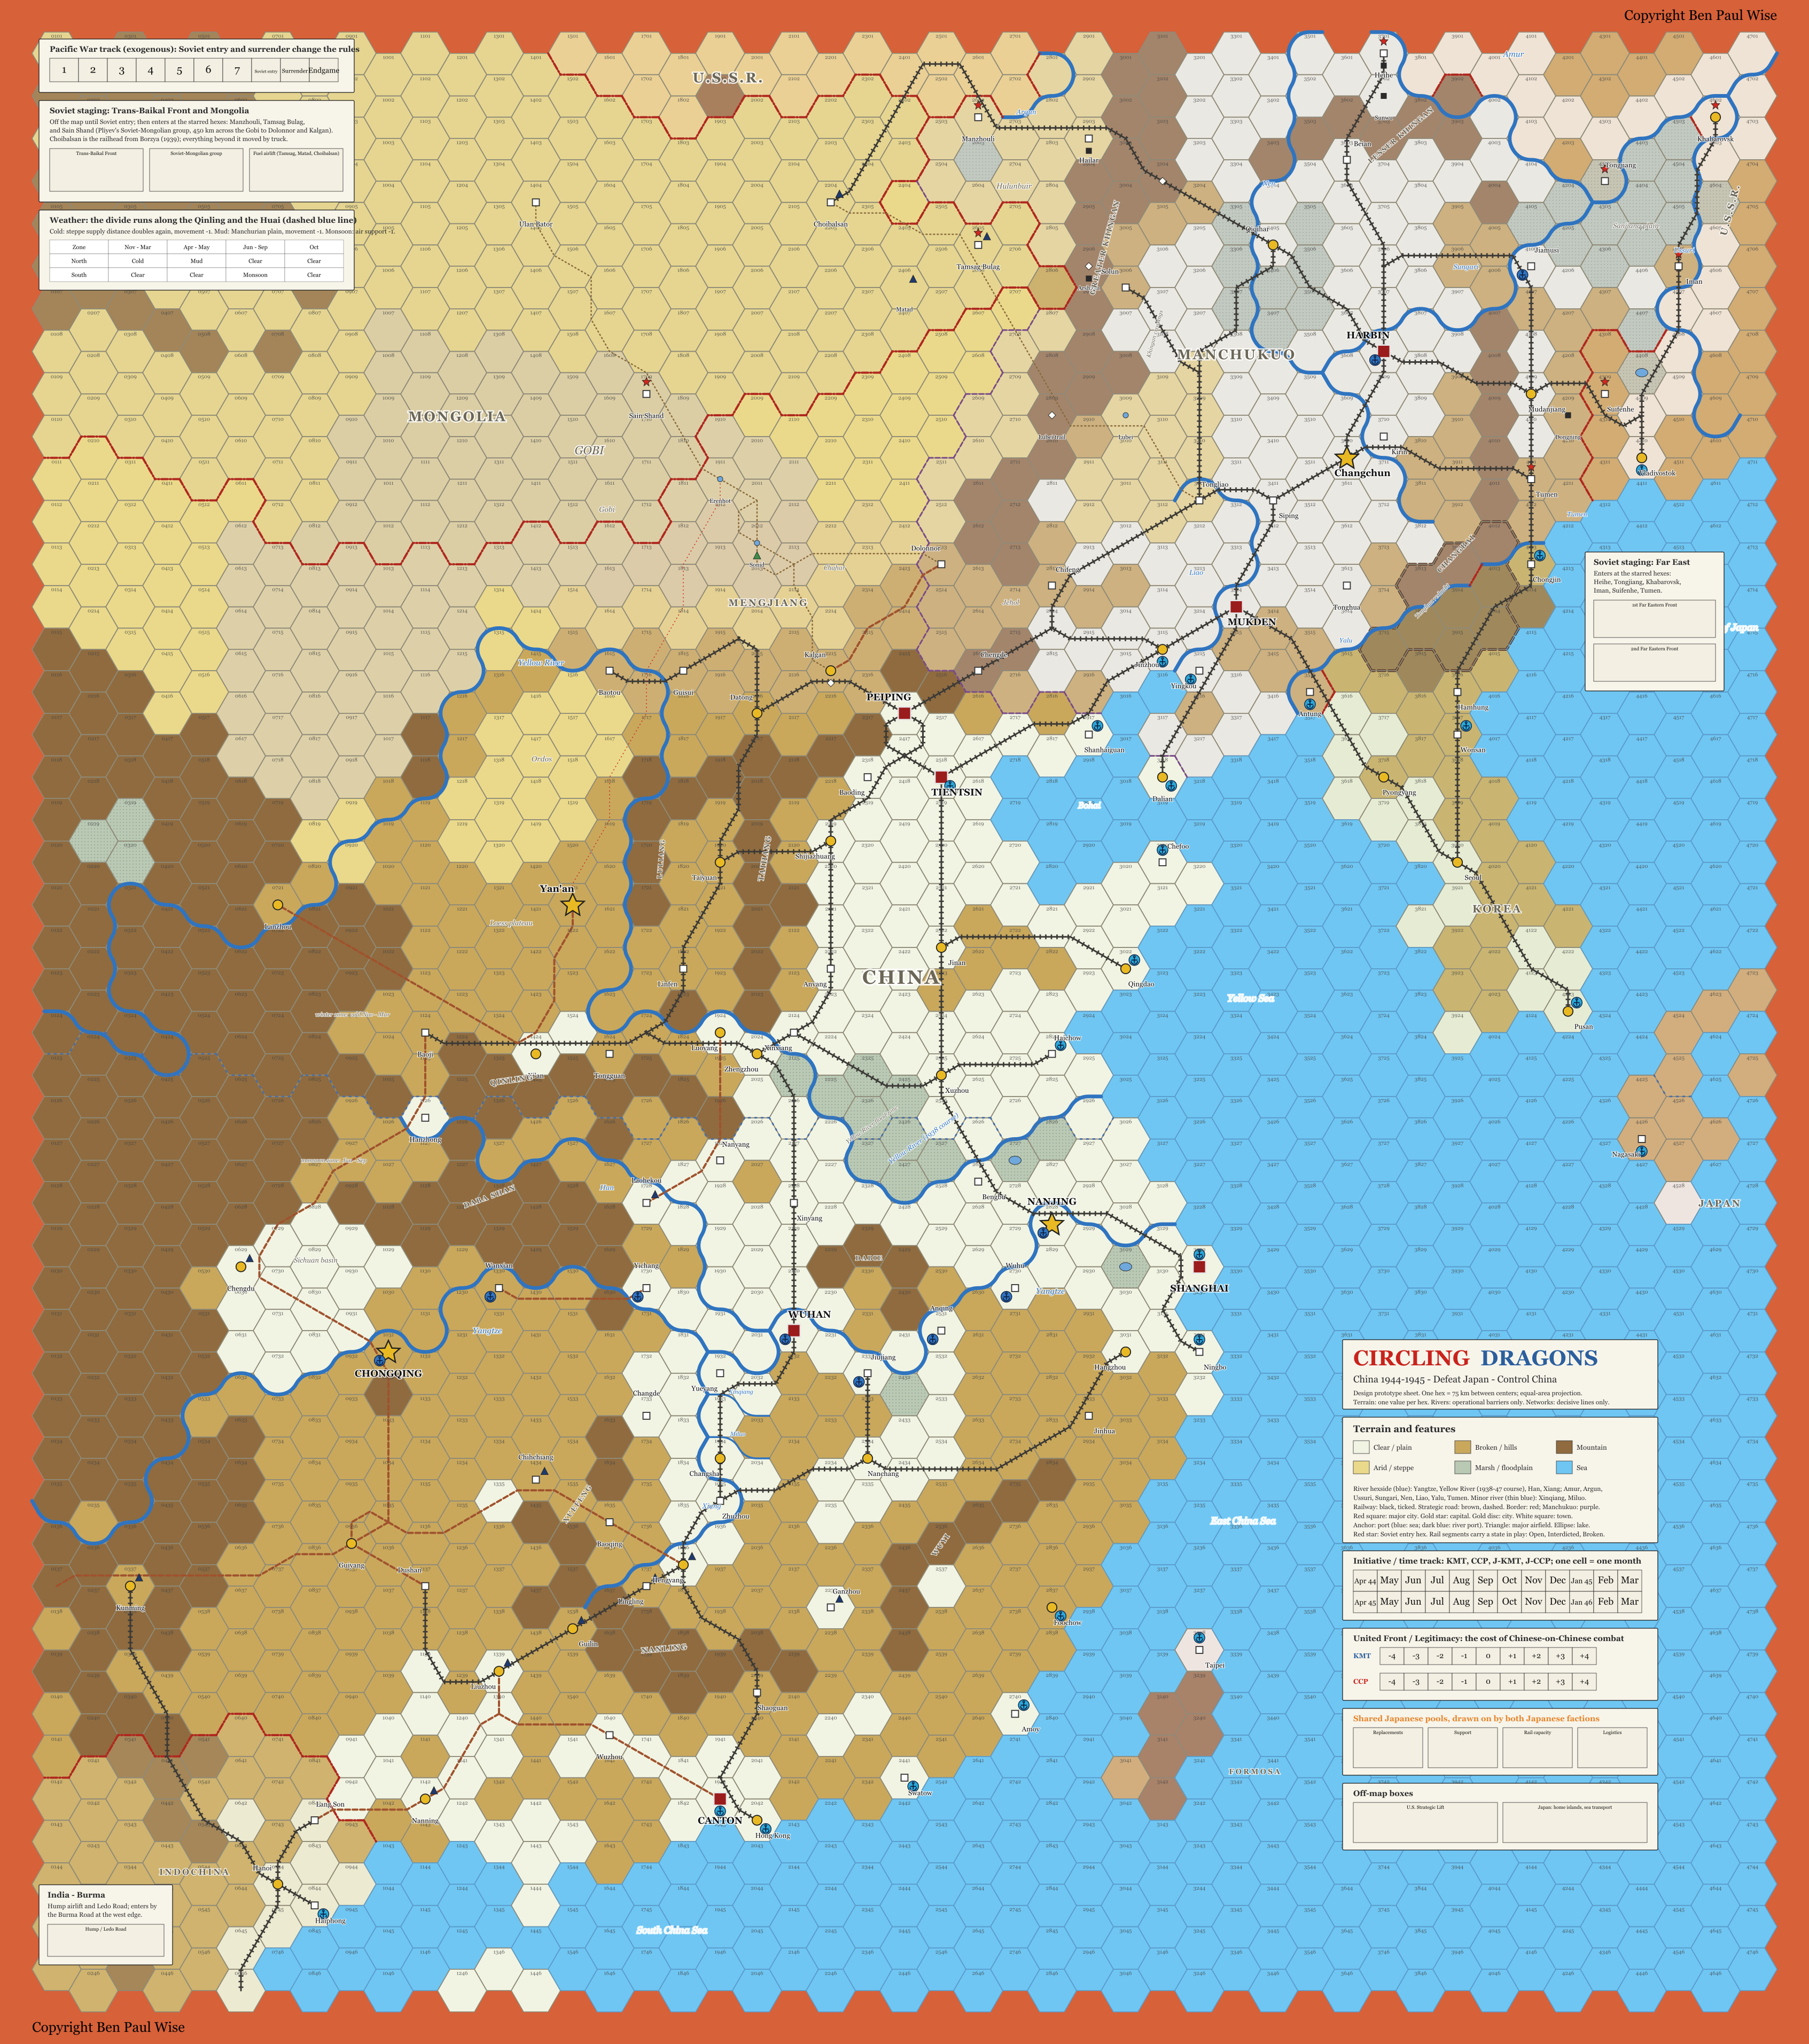
\includegraphics[width=\textwidth,height=.86\textheight,keepaspectratio]{../map_graphics/xml/circling-dragons.png}
\caption{The standard sheet, 75 km between hex centers. The furniture panels keep their size and their places in the corners where little fighting took place; the Mongolian features and the political layer are those of the first sheet.}
\end{figure}
% Copyright Ben Paul Wise. All Rights Reserved.


\subsection{Terrain}\label{sub:terrain}
The map uses five terrain types, \textbf{clear (plain), broken (hills), mountain, marsh (floodplain), and steppe}, with \textbf{desert}, the waterless Gobi and Alashan drawn in a duller sand, as a variant of steppe, and \textbf{sea}. Forest is normally included in broken or mountain terrain. The objective is operational canalization, not tactical simulation. Table \ref{tab:terrain} gives the cost of each terrain class for movement (section \ref{sub:move}), its effect on fire (section \ref{sub:combat}) and its cost to a supply path (section \ref{sub:supply}). \ptest{15}

\begin{table}[ht]
\centering\small
\begin{tabular}{@{}>{\raggedright\arraybackslash}p{.27\textwidth}>{\raggedright\arraybackslash}p{.28\textwidth}>{\raggedright\arraybackslash}p{.20\textwidth}>{\raggedright\arraybackslash}p{.15\textwidth}@{}}
\toprule
Terrain or hexside & Movement cost & Fire into the hex & Supply path cost \\
\midrule
Clear & 1 & --- & 1 \\
Broken & 1 & by motorized pieces at half & 1 \\
Mountain & 2 & at half & 2 \\
Marsh & 2 & by motorized pieces at half & 2 \\
Steppe & 1 & --- & 2 \\
Desert & 2; motorized pieces only along a track & --- & 3 \\
Sea & by Strategic Lift or junk crossing only & --- & closed \\
Fortified city or fortified zone & as its terrain & at half & as its terrain \\
\midrule
Minor river (hexside) & 1 extra & --- & --- \\
Major river (hexside) & 2 extra & across it at half & --- \\
Railway, strategic road or track & 0.5 per edge along it & --- & network (no track) \\
\bottomrule
\end{tabular}
\caption{Terrain and hexsides: movement, fire and supply}\label{tab:terrain}
\end{table}

\paragraph{Rivers.} Rivers run along hexsides. The map prints the \textbf{Yellow River} and the \textbf{Yangtze} as major barriers, and the Han and the Xiang where they shape campaign corridors. In Manchuria, the \textbf{Amur, Ussuri, Sungari (Songhua), Nen, Liao, and Argun} systems matter because they define floodplains, crossings and operational axes. Minor tributaries are represented by terrain costs, with one exception: the standard sheet prints two \textbf{minor rivers}, the Xinqiang and the Miluo north of Changsha, because they were the delay lines of the Changsha battles (section \ref{sub:sheet75}).

\paragraph{Mountains and passes.} The map makes the \textbf{Taihang}, the \textbf{Qinling and central belt}, the \textbf{Xuefeng}, the \textbf{Nanling and the broken terrain of Guangxi and Guizhou}, the \textbf{Greater Khingan}, the \textbf{Lesser Khingan} and the eastern Manchurian highlands visually obvious. The Xuefeng barrier shaped the 1945 Chihchiang (West Hunan) campaign. The Greater Khingan is especially important (Glantz, \emph{August Storm}): Japanese planning treated it and its few routes as a major barrier, and the Soviet operational surprise depended partly on crossing terrain that the defense underestimated. Only a few passes are named; usually a railway or strategic road crossing a mountain hex represents a pass. The Greater Khingan is crossed only at its marked passes, the Boketu rail tunnel, the Arshaan gap on the Solun line and the Lubei trail, and the Yinshan only at Kalgan (section \ref{sub:mongolia-move}).

\paragraph{Marsh, steppe and desert.} Marsh is rare in China proper but prominent in northeastern Manchuria, especially on the Amur--Ussuri--Sungari floodplain. The steppe and desert of western Manchuria and Mongolia penalize supply more than combat.

\subsection{The transport network}\label{sub:network-map}
The map follows one cartographic rule:
\begin{quote}\textbf{A transportation line is printed only if removing it would change a player's strategic decisions.}\end{quote}

The core rail network includes:
\begin{itemize}
\item \textbf{Peiping--Hankow (Pinghan)}, central to the first phase of Ichi-Go;
\item \textbf{Canton--Hankow and the Hunan corridor}, especially Changsha--Hengyang;
\item \textbf{Hunan--Guangxi}, Hengyang--Guilin--Liuzhou;
\item \textbf{Longhai}, the main east--west trunk of the central plains;
\item \textbf{Tientsin--Pukow (Jinpu, Tsinpu)};
\item \textbf{Peiping--Suiyuan, Datong--Puzhou, and Shijiazhuang--Taiyuan};
\item \textbf{the Manchurian trunks}: Harbin--Changchun--Mukden, the South Manchuria line, Harbin--Qiqihar--Hailar--Manzhouli, and the eastern line through Mudanjiang to Suifenhe; and
\item \textbf{the Shanhaiguan corridor}, the overland gateway between North China and Manchuria.
\end{itemize}

The map does not print a dense road net. It prints only the \textbf{strategic roads} whose existence changes supply or connects otherwise difficult terrain. The Yangtze and the Sungari provide limited strategic transport between designated ports. In Mongolia the map prints dotted \textbf{Gobi tracks}: the Kalgan--Urga road through Erenhot and Sain Shand, the Erenhot--Sonid--Dolonnor trail, the Tamsag Bulag--Lubei trail over the Khingan, and the Choibalsan--Tamsag supply road. Tracks carry movement but are not part of the supply network (section \ref{sub:supply}).

\subsection{Operational nodes}
A city appears on the map if it is a transport junction, a political objective, a major port or airfield, or the base of a campaign (table \ref{tab:nodes}).

\begin{longtable}{p{.23\textwidth}p{.69\textwidth}}
\caption{Operational nodes}\label{tab:nodes}\\
\toprule Node & Map function \\\midrule\endfirsthead
\toprule Node & Map function \\\midrule\endhead
\bottomrule\endfoot
Peiping--Tientsin & Political and transport center; ports and railheads; a principal objective of the 1945 surrender race.\\
Shijiazhuang--Taiyuan & Taihang rail corridor; Japanese occupation and CCP interdiction geography.\\
Zhengzhou & Junction of major north--south and east--west rail axes; objective of the first phase of Ichi-Go.\\
Wuhan & Yangtze transport hub and northern base of the central Ichi-Go corridor.\\
Changsha--Hengyang & Main Hunan corridor; major 1944 fighting and transport and airfield objectives.\\
Guilin--Liuzhou & Southern Ichi-Go rail and airfield objectives.\\
Chihchiang (Zhijiang) & 1945 airfield objective west of the Xuefeng barrier.\\
Chongqing--Chengdu & KMT political and rear-area center, near the western edge of the map.\\
Yan'an & CCP political and base node rather than conventional logistics hub.\\
Shanghai--Nanjing & Political, industrial, port and rail objectives.\\
Qingdao and the North China ports & Strategic entry points for post-surrender transport.\\
Shanhaiguan--Qinhuangdao & Narrow gateway and rail connection into Manchuria.\\
Mukden, Changchun, Harbin & Principal central and southern Manchurian political and rail hubs.\\
Qiqihar, Hailar--Manzhouli & Northwestern communications and approach nodes.\\
Mudanjiang--Suifenhe & Eastern road and rail axis and major Soviet--Japanese corridor.\\
Dalian--Port Arthur; Huludao--Yingkou & Ports affecting entry into southern Manchuria.\\
\end{longtable}

\subsection{Mongolia and the Soviet entry hexes}\label{sub:mongolia-map}
Outer Mongolia is on the map but out of the war until Soviet entry. Nothing happened there in 1944--45 except preparation: eastern Mongolia was the Trans-Baikal Front's staging ground, with the railhead at Choibalsan (the Borzya line of 1939) and the forward depots at Tamsag Bulag, and everything beyond them moved by truck. The map marks the \textbf{Soviet entry hexes} with a red star: Manzhouli, Tamsag Bulag and Sain Shand on the western side; Heihe, Tongjiang and Khabarovsk on the Amur; Iman, Suifenhe and Tumen on the eastern side. It also marks the \textbf{water points} (Erenhot, Sonid, Lubei, Sain Shand), the fuel-airlift airfields (Tamsag Bulag, Matad and Choibalsan), the passes of the Greater Khingan, and the six \textbf{Kwantung Army fortified zones} (Hailar, Aihui, Sunwu, Arshaan, Hutou, Dongning).

\subsection{The political layer}
The map carries a second, lightly drawn layer over the north: Mengjiang as a light wash over Chahar and Suiyuan, the Inner Mongolian autonomy marker at Sonid, the Tonghua redoubt outlined along the Korean border, the weather divide along the Qinling and the Huai, and a faint liaison route from Yan'an across the Ordos. Its rules are provisional (section \ref{sub:political}).

\subsection{Markers}\label{sub:markers}
The markers record control and the state of the map. A marker with two states carries one on each face: presence and base area, KMT and CCP control, rail interdicted and broken, port denied and open, airfield captured and destroyed, and the front a Japanese formation faces. Other markers are the fortified cities and the bridge markers (e.g., the Yellow River rail bridge at Zhengzhou), the Japanese directives, the fuel airlift, halted and withdrawal markers of the Soviet groupings, Soviet occupation markers, surrendered-garrison markers, the US Marines as port markers, and the markers of the tracks and pools.

% ======================================================================================================================
% Part 4: pieces
% ======================================================================================================================
\section{Pieces}\label{sec:pieces}
\subsection{Kinds of pieces}
\begin{itemize}
\item \textbf{Unit pieces} are formations with combat values: Japanese divisions, independent mixed brigades, railway garrisons and headquarters; Kwantung Army and Korea Army pieces; KMT group armies, US-equipped armies and headquarters; CCP field forces, Northeast columns and headquarters; Soviet groupings; and puppet armies. The tank formations and the cavalry-mechanized group are \textbf{motorized}; all others move \textbf{on foot}.
\item \textbf{Air-support pieces} stand for the air forces, e.g., the US Fourteenth Air Force. They do not fire; they support combat and supply air-supplied hexes (sections \ref{sub:air-combat} and \ref{sub:air-supply}).
\item \textbf{Supply pieces} carry supply forward along the network (section \ref{sub:supply}). They have no combat values and count as markers for stacking.
\item \textbf{Markers} record information (section \ref{sub:markers}). CCP presence markers, whose backs are base areas, are markers, not pieces.
\end{itemize}

\subsection{Counts by faction}\label{sub:counts}
The counts in table \ref{tab:counts} are an estimate, taken from \emph{Downfall}'s density of pieces per hex in play, and the prototype will revise them. \emph{Downfall} prints about 800 land hexes in play and opens with about 90 land pieces on the map, one per nine hexes, rising to about 110 at its peak; its 3--4 step unit is an army, its 2-step unit a corps, its 1-step unit a division. The first estimate, made for the 100 km sheet's 672 hexes in play, was 72 unit pieces and about 200 counters; for the 75 km sheet the set was grown to 126 unit pieces.

\begin{table}[ht]
\centering\small
\begin{tabular}{@{}lrp{.62\textwidth}@{}}
\toprule Faction & Pieces & What a piece is \\\midrule
Japan & 51 & China Expeditionary Army: 24 division pieces of 3 steps (23 infantry and the 3rd Tank Division), 4 pieces of independent mixed brigades, 7 one-step railway garrisons, and 3 headquarters, the area army a formation answers to deciding the front it faces; Kwantung Army 10 pieces of 2 steps, two for each of its five armies; Korea 3. Reinforced by event in 1945.\\
KMT & 35 & 24 group-army pieces of 2--3 steps and uneven quality, 6 of them regional troops; 5 US-equipped armies, 2 of them in Burma at the start; 2 Y-Force group armies returning from Burma in 1945; 4 headquarters.\\
CCP & 23 & 16 field forces of 2 steps (Eighth Route Army 8, New Fourth Army 7, South China 1); 5 Northeast columns formed in play by concentration of presence; 2 headquarters. Also 24 presence markers whose backs are base areas, which are not pieces.\\
Soviet & 11 & scripted groupings entering in August 1945.\\
Puppets & 6 & Nanjing regime 3, Manchukuo 2, Mengjiang 1; one step each, passing at the surrender.\\
\bottomrule
\end{tabular}
\caption{Unit pieces by faction}\label{tab:counts}
\end{table}

About 105 of the 126 unit pieces are on the map at the start, one to 11 hexes in play; with the Soviets and the Northeast columns the peak is 126, one to 9.4 hexes, \emph{Downfall}'s density. The piece is therefore \emph{Downfall}'s 2- and 3-step corps-level unit, not its army: at army scale Japan would field 12 pieces and the KMT's twelve war areas 12, too thin for a 47 by 46 sheet. With 5 air-support pieces, 13 supply pieces and the markers the counter set comes to 263, against \emph{Downfall}'s 351. \textbf{Preliminary:} every figure here is to be tested, in particular whether the CCP presence layer stays legible (section \ref{sub:open}).

\subsection{Values}\label{sub:pieces}
Table \ref{tab:pieces} gives each kind of unit piece its offense, defense, allowance and steps. The offense is the strength printed on the counter now. The defense is new: one more than the offense for KMT group armies and railway garrisons, which held ground better than they attacked; one less for the tank formations and the cavalry-mechanized group, after the HexKrieg armor (offense 8, defense 6); equal to the offense otherwise. \ptest{10}

\begin{table}[ht]
\centering\small
\begin{tabular}{@{}lrrrrrl@{}}
\toprule
Piece & Pieces & Offense & Defense & Allowance & Steps & Class \\
\midrule
Japanese infantry division & 23 & 3 & 3 & 4 & 3 & foot \\
Japanese 3rd Tank Division & 1 & 4 & 3 & 6 & 3 & motorized \\
Japanese independent mixed brigade & 4 & 1 & 1 & 3 & 1 & foot \\
Japanese railway garrison & 7 & 1 & 2 & 2 & 1 & foot \\
Kwantung Army piece & 10 & 2 & 2 & 4 & 2 & foot \\
Korea Army piece & 3 & 2 & 2 & 3 & 2 & foot \\
Puppet army (Mengjiang allowance 3) & 6 & 1 & 1 & 2 & 1 & foot \\
KMT group army, regular & 18 & 2 & 3 & 3 & 3 & foot \\
KMT group army, regional troops & 6 & 1 & 2 & 3 & 2 & foot \\
KMT US-equipped army & 5 & 4 & 4 & 4 & 3 & foot \\
KMT Y-Force group army & 2 & 3 & 3 & 3 & 3 & foot \\
CCP field force or Northeast column & 21 & 2 & 2 & 4 & 2 & foot \\
Headquarters (Japanese 3, KMT 4, CCP 2) & 9 & 0 & 1 & 4 & 1 & foot \\
Soviet 6th Guards Tank Army & 1 & 6 & 5 & 8 & 4 & motorized \\
Soviet 39th, 5th and 1st Red Banner Armies & 3 & 4 & 4 & 5 & 4 & foot \\
Soviet armies of three steps & 6 & 3 & 3 & 5 & 3 & foot \\
Soviet cavalry-mechanized group (Pliyev) & 1 & 3 & 2 & 8 & 3 & motorized \\
\bottomrule
\end{tabular}
\caption{Unit pieces: offense, defense, allowance and steps}\label{tab:pieces}
\end{table}

\subsection{Steps}\label{sub:steps}
A unit piece has one to four steps. Its back face shows it reduced, and a step marker shows a loss short of the back face. A piece's current offense and defense are its values multiplied by the fraction of its steps that remain; e.g., a Japanese division with two of its three steps has offense 2 and defense 2. Fractions are kept. A piece that loses its last step is removed.

\subsection{Supply pieces}\label{sub:supply-pieces}
\ptest{3} The counter set carries 13 supply pieces at the placeholder counts: Japanese \texttt{jp-supply1} to \texttt{jp-supply6} in China and \texttt{kw-supply1} and \texttt{kw-supply2} in Manchuria and Korea, and KMT \texttt{kmt-supply1} to \texttt{kmt-supply5}. The Soviets and the CCP have none. Section \ref{sub:supply} gives their rules.

% ======================================================================================================================
% Part 5: sequence of play
% ======================================================================================================================
\section{Sequence of play}\label{sec:sequence}
\subsection{The time track and initiative}\label{sub:timetrack}
There are four initiative markers:
\[
KMT,\qquad CCP,\qquad J_{KMT},\qquad J_{CCP},
\]
where $J_{KMT}$ is the Japanese faction facing the KMT, commanded by the CCP player, and $J_{CCP}$ the Japanese faction facing the CCP, commanded by the KMT player. The faction furthest behind on the time track normally acts next. Orders consume different amounts of time. Calendar thresholds trigger seasonal effects and dated strategic events. One calendar interval is approximately one month. After the surrender the endgame is played in initiative rounds, which set the timing of the race (section \ref{sub:surrender}). The time each order costs is not yet fixed (draft in appendix \ref{app:orders}).

\subsection{Orders}\label{sub:orders}
The menu of orders is short: \textbf{Move/Redeploy, Attack, Move--Attack, Rail Redeploy, Recover/Refit, Political/Base Action,} and \textbf{Interdict/Repair Transport}. Japanese strategic directives restrict the objectives their operations may pursue without dictating the exact move (section \ref{sub:directives}).

\subsection{The activation}\label{sub:activations}
When the time track activates a faction, the faction gives its orders. Sections 6 to 8 govern Move, Attack, Move--Attack and Recover/Refit. Rail Redeploy and Interdict/Repair Transport are given in section \ref{sub:rail}, and Political/Base Action in section \ref{sub:presence}. An activation proceeds in this order.
\begin{enumerate}
\item The pieces with Move or Move--Attack orders move, one at a time (section \ref{sub:move}).
\item The faction declares its attacks: each attacking piece names one adjacent enemy hex (section \ref{sub:combat}).
\item Each defending piece that qualifies may withdraw before combat.
\item All declared attacks and the return fire are resolved together, with the strengths at the moment of declaration.
\item The results are applied: retreats, then step losses, then assault losses, then advances.
\item Supply levels are computed for every piece on the map (section \ref{sub:supply}), attrition is applied, and pieces that refitted recover (section \ref{sub:recovery}).
\end{enumerate}
A piece with an Attack order attacks without moving; a piece with a Move--Attack order may attack after it moves.

\subsection{The calendar}\label{sub:calendar}
Dated events on the calendar and on the Pacific War track change the game: the arrival of reinforcements (section \ref{sub:reinforcements}), the seasons (section \ref{sec:weather}), the Soviet entry (historically 8 and 9 August 1945, section \ref{sub:soviet}), the Sino-Soviet treaty (historically 14 August 1945, section \ref{sub:treaty}), and the Japanese surrender (historically 15 August 1945, section \ref{sub:surrender}). Entry is a dated or conditional strategic event, and the scenario gives the dates.

% ======================================================================================================================
% Part 6: movement
% ======================================================================================================================
\section{Movement}\label{sec:movement}
\subsection{Land movement}\label{sub:move}
\paragraph{Edge costs.} Movement is on the edges between hex centers, as in HexKrieg. The cost of the edge from hex $h$ to an adjacent hex $h'$ is
\begin{eqnarray}
c(h,h') &=& \tfrac{1}{2}\left(t(h)+t(h')\right)+s(h,h') \mbox{\quad off the transport lines,} \label{eq:edge_A}\\
c(h,h') &=& 0.5 \mbox{\quad along a railway, strategic road or track,} \label{eq:edge_B}
\end{eqnarray}
where $t$ is the terrain cost of table \ref{tab:terrain} and $s$ the surcharge of a river on the hexside between $h$ and $h'$. An edge along a line joins two consecutive hexes of the same railway, road or track; a river under it is bridged and adds nothing, unless a marker shows the bridge down (e.g., the Yellow River rail bridge at Zhengzhou). \ptest{15}

\paragraph{Example.} The move of \texttt{jp-d40} in Changsha a2, from 2032 to 2033 to 2034, crosses the Xinqiang and then the Miluo; by equation \eqref{eq:edge_A} each edge costs $1+1=2$, and the move costs 4 points.

\begin{enumerate}
\item \textbf{Allowance.} A moving piece pays the cost of each edge from its allowance (equations \eqref{eq:edge_A} and \eqref{eq:edge_B}) and stops when it cannot pay for the next edge. A piece that has not moved in the activation may always move one hex, into any hex it may enter. Supply may reduce the allowance of motorized pieces (table \ref{tab:supply}).
\item \textbf{Prohibited hexes.} A piece may not enter a hex an enemy piece holds, nor a sea hex except by Strategic Lift or junk crossing (section \ref{sub:sea-move}). No Chinese or Japanese formation may enter a Mongolian hex (section \ref{sub:mongolia-move}). A motorized piece enters a desert hex only along a track.
\item \textbf{Zones of control.} \ptest{14} A piece's zone of control is the six hexes around it, except a hex across a major river and a mountain hex; a minor river does not block it. A piece that enters a hex in an enemy zone stops there. A piece that begins its move in an enemy zone may leave it with its first step and continues normally after that. Zones of control also block supply paths (section \ref{sub:supply}).
\item \textbf{Stacking.} At the end of each step a hex may hold two unit pieces, any number of markers and one air-support piece; a surrendered Japanese piece does not count. A step that would exceed the limit is not taken, and the piece stops.
\item \textbf{Enemies.} \ptest{16} Japanese pieces of either controller are enemies of KMT, CCP and Soviet pieces. KMT and CCP pieces exert no zone of control on each other and fight only in an attack a player declares at the Legitimacy cost (section \ref{sub:civil}).
\end{enumerate}

\subsection{Rail redeployment and the state of the railways}\label{sub:rail}
\paragraph{Rail Redeploy.} A Rail Redeploy order moves pieces along open railway; it draws on the shared rail capacity when the pieces are Japanese (section \ref{sub:directives}). A piece may not rail-redeploy into or out of a hex in an enemy zone of control. The capacity and the time cost of the order are not yet fixed (draft in appendices \ref{app:orders} and \ref{app:rail}).

\paragraph{Rail state.} Rail segments have three states:
\begin{enumerate}
\item \textbf{Open}: supply and strategic redeployment allowed.
\item \textbf{Interdicted}: supply possible with penalty; strategic redeployment blocked or costly.
\item \textbf{Broken}: unusable until repaired.
\end{enumerate}
The Interdict/Repair Transport order changes the state of a segment, and a marker shows it. CCP presence makes interdiction comparatively easy (section \ref{sub:presence}); secure conventional occupation is needed to keep major junctions reliably open. The penalty of an interdicted segment for supply is not yet fixed (draft in appendix \ref{app:rail}).

\subsection{Mongolia and the Soviet groupings}\label{sub:mongolia-move}
\begin{enumerate}
\item \textbf{Sanctuary.} No Chinese or Japanese formation may enter a Mongolian hex. Soviet formations use Mongolian hexes freely. The border therefore has a function in the rules.
\item \textbf{Entry and axes.} At Soviet entry the groupings appear at their stars and follow fixed axes (section \ref{sub:soviet}). The western axes are Manzhouli--Hailar--Qiqihar; Tamsag Bulag over the Greater Khingan to Tongliao, Mukden and Changchun; and Sain Shand over the Gobi to Dolonnor and the Kalgan gap (Pliyev's Soviet--Mongolian cavalry-mechanized group, some 450 km of desert in ten days). The Gobi tracks print these axes. In a desert hex a motorized grouping moves and traces supply only along a track.
\item \textbf{Passes.} The Greater Khingan is crossed only at its marked passes, the Boketu rail tunnel, the Arshaan gap on the Solun line and the Lubei trail, and the Yinshan only at Kalgan.
\item \textbf{Halts.} A Soviet motorized grouping may be halted for lack of fuel, and the cavalry group for lack of water (section \ref{sub:steppe-supply}).
\end{enumerate}

\subsection{Sea and river movement}\label{sub:sea-move}
There are no naval pieces and no naval combat. Movement by sea is of three kinds.
\begin{itemize}
\item \textbf{Strategic Lift.} U.S. transport support is abstract. A limited Strategic Lift resource can relocate KMT formations between eligible air, port and rail nodes. After the surrender it moves KMT armies by air and sea, and the ports a lift may use depend on the Sino-Soviet treaty (section \ref{sub:treaty}).
\item \textbf{Junk crossing.} The CCP may cross the Bohai by junk, as the Shandong forces did in 1945. The capacity and the time cost are not yet fixed (draft in appendix \ref{app:junks}).
\item \textbf{River transport.} The Yangtze and the Sungari provide limited strategic transport between designated ports.
\end{itemize}

\subsection{Air movement}\label{sub:air-move}
Air-support pieces act within four hexes of their position, in combat (section \ref{sub:air-combat}) and in supply (section \ref{sub:air-supply}). How they move between airfields is not yet written (draft in appendix \ref{app:air}). The KMT divisions flown back from Burma in December 1944 arrive by air at Kunming (section \ref{sub:reinforcements}), and the Soviet fuel airlift is a pool drawn down from the airfields at Tamsag Bulag, Matad and Choibalsan (section \ref{sub:steppe-supply}). There are no airborne rules: the Soviet airborne detachments of August 1945 appear in the figures in the cities, and their rule is not yet written.

% ======================================================================================================================
% Part 7: combat
% ======================================================================================================================
\section{Combat}\label{sec:combat}
\subsection{Land combat}\label{sub:combat}
\begin{enumerate}
\item \textbf{Attacks.} Each piece of the active faction that has an Attack or Move--Attack order and is adjacent to an enemy hex may attack one adjacent enemy hex. Its modified offense is split evenly among the enemy pieces in that hex, one fire stream to each.
\item \textbf{Return fire.} Each attacked piece returns fire at the pieces attacking it: all of its modified offense at one attacker, half at each of two, or half at each of two chosen at random among three or more, as in HexKrieg. A piece supplied only by air returns fire but may not attack.
\item \textbf{Withdrawal before combat.} \ptest{13} A defending piece in broken or mountain terrain, or with a river hexside between it and every adjacent enemy piece, may withdraw one hex when an enemy piece moves adjacent to it or declares an attack on it. It may not withdraw into a hex an enemy piece holds, nor into an enemy zone unless a friendly piece holds that hex. Its faction's marker moves one space on the time track. Fire aimed at the piece is lost, and its attackers may advance into its hex.
\item \textbf{Modifiers.} The following multiply a fire stream, and all of them apply together.
\begin{itemize}
\item A piece that receives fire streams across two hexsides that are not adjacent to each other (e.g., from the north and from the southeast) has every stream it receives raised by half.
\item Fire into a mountain hex is halved, and fire by a motorized piece into a broken or marsh hex is halved.
\item Fire across a major river hexside is halved, in attack and in return fire. \ptest{12}
\item Fire into a fortified city or a Kwantung fortified zone is halved.
\item Air support raises its side's streams by half (section \ref{sub:air-combat}). \ptest{11}
\end{itemize}
Offense and defense are also multiplied by the supply multipliers of table \ref{tab:supply} and by the fraction of the piece's steps that remain.
\item \textbf{Odds.} \ptest{9} For each defending piece, $A$ is the sum of the modified streams it receives and $D$ its modified defense. The odds are rounded in the defender's favor:
\begin{eqnarray}
R &=& \left\lfloor A/D \right\rfloor \mbox{\quad giving odds } R{:}1, \mbox{ when } A \ge D, \label{eq:odds_A}\\
R &=& \left\lceil D/A \right\rceil \mbox{\quad giving odds } 1{:}R, \mbox{ when } A < D. \label{eq:odds_B}
\end{eqnarray}
HexKrieg rounds both ratios up from three quarters,
\begin{eqnarray}
R &=& \left\lfloor \tfrac{1}{4}+A/D \right\rfloor \mbox{\quad when } A \ge D, \label{eq:hkodds_A}\\
R &=& \left\lfloor \tfrac{1}{4}+D/A \right\rfloor \mbox{\quad when } A < D, \label{eq:hkodds_B}
\end{eqnarray}
so that by equation \eqref{eq:hkodds_B} an attack of 2 on a defense of 3 counts as 1:1; by equation \eqref{eq:odds_B} it counts as 1:2.
\item \textbf{The table.} One ten-sided die is rolled for each defending piece and read on table \ref{tab:crt}. The results apply to the defending piece only; attackers suffer only what the return fire does to them.
\item \textbf{Results.} NR: no result. R: the piece retreats one hex, not into or through a hex an enemy piece holds, not into a sea hex and not beyond the stacking limit; enemy zones do not bind a retreat. If no hex is open, the piece loses one step instead. A piece in a fortified city or a fortified zone may refuse a retreat and lose one step instead. S: the piece loses one step. E: the piece loses two steps, which eliminates a piece of one or two steps.
\item \textbf{Assault losses.} \ptest{8} After the results, if a fortified city or a fortified zone that was attacked is still held by a defending piece, one ten-sided die is rolled for each piece that attacked it; on 8, 9 or 10 that piece loses one step. The roll is separate from the return fire, which still applies.
\item \textbf{Advance.} After the results, attacking pieces adjacent to a hex that combat or withdrawal has emptied may enter it, within the stacking limit, and stop there. When enemy pieces enter a fortified city, its marker is removed.
\end{enumerate}

\begin{table}[ht]
\centering\small
\begin{tabular}{@{}l*{10}{c}l@{}}
\toprule
Odds & 1 & 2 & 3 & 4 & 5 & 6 & 7 & 8 & 9 & 10 & HexKrieg row used \\
\midrule
1:4 or less & NR & NR & NR & NR & NR & NR & NR & NR & NR & NR & none (new) \\
1:3 & NR & NR & NR & NR & NR & NR & NR & NR & NR & R & 1:5 or less \\
1:2 & NR & NR & NR & NR & NR & NR & NR & R & R & S & none (new) \\
1:1 & NR & NR & NR & NR & R & R & R & S & S & E & 1:2 \\
2:1 & NR & NR & NR & R & R & R & S & S & S & E & 1:1 \\
3:1 & NR & NR & R & R & R & S & S & S & E & E & 2:1 \\
4:1 & NR & R & R & R & S & S & S & E & E & E & 3:1 \\
5:1 & R & R & R & S & S & S & E & E & E & E & 4:1 \\
6:1 or more & R & R & S & S & S & E & E & E & E & E & 5:1 or more \\
\bottomrule
\end{tabular}
\caption{Combat table, effects on the defending piece; columns are the roll of one ten-sided die}\label{tab:crt}
\end{table}

\paragraph{Example: the fall of Hengyang (b4).} \texttt{jp-d58} fires from 1835 across the Xiang, $3\times\tfrac{1}{2}=1.5$, and \texttt{jp-d13} from 1937, 3: together 4.5. The streams arrive across the north and southeast hexsides, which are not adjacent, so they are raised by half to 6.75, and the fortified city halves them to 3.375. The garrison, \texttt{kmt-ga10} with one step of three and at supply level 1 by air, has defense $3\times\tfrac{1}{3}\times 0.85=0.85$. Then $A/D=3.97$, and by equation \eqref{eq:odds_A} the odds are 3:1: on rolls of 3 to 10 the garrison retreats if a hex is open, or is eliminated.

\subsection{Fortified cities and fortified zones}\label{sub:fortified}
The rules for fortified cities and the Kwantung Army's fortified zones are gathered here.
\begin{itemize}
\item Fire into a fortified city or fortified zone is halved (section \ref{sub:combat}, item 4).
\item A piece in one may refuse a retreat by losing one step (item 7).
\item Each piece that attacks one without taking it may suffer an assault loss (item 8). \ptest{8}
\item When enemy pieces enter a fortified city, its marker is removed (item 9).
\item A piece in a fortified city may be supplied by air (section \ref{sub:air-supply}).
\item A Kwantung Army fortified zone (Hailar, Aihui, Sunwu, Arshaan, Hutou, Dongning) holds a Soviet grouping that attacks it for one activation; a bypassed zone keeps its hex until the general surrender, as Hutou did until 26 August 1945.
\end{itemize}

\subsection{Chinese-on-Chinese combat}\label{sub:civil}
Direct KMT--CCP combat is possible but politically expensive. A \textbf{United Front (Legitimacy) track} imposes costs in political standing, external support, or victory position. This makes indirect damage inflicted by Japanese forces attractive without forbidding historically plausible clashes. Before the surrender KMT and CCP pieces exert no zones of control on each other \ptest{16}; they fight only when a player declares an attack and pays the Legitimacy cost. The size of the cost is a placeholder (draft in appendix \ref{app:legit}).

\subsection{Air combat and air support}\label{sub:air-combat}
There is no air-to-air combat. \ptest{11} Provisionally, one air-support piece within four hexes may support one combat per activation, its side's attack or its side's defense; that side's streams in the combat are raised by half. Air-support pieces may also attack bridges (e.g., the Fourteenth Air Force against the Yellow River bridge at Zhengzhou in 1944); the effect is not yet written (draft in appendix \ref{app:air}). Captured and destroyed airfield markers record the loss of air support.

\subsection{Naval combat}
There is no naval combat. Sea power enters the game through Strategic Lift, the ports and the junk crossings (section \ref{sub:sea-move}).

% ======================================================================================================================
% Part 8: supply
% ======================================================================================================================
\section{Supply}\label{sec:supply}
\subsection{Land supply}\label{sub:supply}
Supply runs from sources along the transport network, relayed by supply pieces, and from the network to each piece by a short local path. Mountain, marsh and arid terrain sharply restrict supply off the network, and supply matters more than small terrain combat modifiers.
\begin{enumerate}
\item \textbf{Sources.} The scenario names each faction's supply sources: ports, capitals, depots and railheads, and the base areas of the CCP. Sources do not move.
\item \textbf{Network.} A faction's network is the railway, strategic road and river-route hexes that no enemy piece holds and that are not in an enemy zone of control unless a friendly piece holds them. Tracks are not part of the network. Distances along the network are counted in hexes, along one line or from one line to another where they share a hex. The hex of a source counts as a network hex.
\item \textbf{Supply pieces.} \ptest{3} \ptest{5} A supply piece is a counter without combat values; it counts as a marker for stacking. It moves only along its faction's network, by a Move order (allowance 4, at 0.5 per edge) or by Rail Redeploy, and may not enter a hex in an enemy zone unless a friendly unit piece holds it. If an enemy piece enters its hex, it is removed. Japanese supply pieces belong to a front, like Japanese formations, and are moved by that front's controller.
\item \textbf{Reach and coverage.} \ptest{1} \ptest{2} The reach $R$ is a number of network hexes, set by play testing; the first value to test is 6. A source covers at level 3 every network hex within $R$ hexes of it along the network. A supply piece on a covered hex relays supply: it covers every network hex within $R$ hexes of it at one level less than the level of its own hex, the loss per relay of the supply draft. A hex covered more than once takes the highest level offered.
\item \textbf{Local path.} A piece off the network traces a local path to a covered network hex. The path may not enter a sea hex, a hex an enemy piece holds, or a hex in an enemy zone unless a friendly piece holds it. Its cost is the sum, over the hexes it enters (the network hex included), of the supply path costs of table \ref{tab:terrain}. A piece on a network hex has a cost of 0.
\item \textbf{Level.} \ptest{7} A local path costing 3 or less allows level 3; 4 or 5, level 2; 6 or 7, level 1. A piece's level is the lower of the two numbers, the coverage level of the hex its path reaches and the level its path allows, taking the best such hex it can reach. A piece with no such path is at level 0.
\item \textbf{The CCP.} \ptest{4} The CCP has no supply pieces. Its base areas are its sources, and its field forces trace their local paths to them. CCP dispersed presence uses this lighter support rule and does not require an unbroken conventional rail chain.
\item \textbf{Long reach.} If $R$ exceeds every distance on the sheet, the sources cover their whole connected network at level 3, supply pieces are never needed, and a piece's level depends on its local path alone. That is a plain trace along the network.
\item \textbf{Multipliers.} \ptest{7} Table \ref{tab:supply} gives the multipliers of each level. Allowances are rounded to the nearest whole point and are never below 1.
\item \textbf{Attrition.} A piece at level 0 at the end of two consecutive activations of its own faction loses one step at the end of the second.
\item \textbf{Timing.} Levels are computed at the end of every activation for every piece on the map and are used until the end of the next activation, the one-cycle delay of the supply draft.
\end{enumerate}

\begin{table}[ht]
\centering\small
\begin{tabular}{@{}lrrrr@{\qquad}rrr@{}}
\toprule
& \multicolumn{4}{c}{\emph{Circling Dragons}} & \multicolumn{3}{c}{HexKrieg draft} \\
Level & Offense & Defense & Allowance, foot & Allowance, motorized & Offense & Defense & Movement \\
\midrule
3 & 1.00 & 1.00 & 1.00 & 1.00 & 1.00 & 1.00 & 1.00 \\
2 & 0.75 & 1.00 & 1.00 & 0.85 & 0.70 & 0.90 & 0.85 \\
1 & 0.50 & 0.85 & 1.00 & 0.65 & 0.40 & 0.75 & 0.65 \\
0 & 0.50 & 0.75 & 1.00 & 0.40 & 0.15 & 0.55 & 0.40 \\
\bottomrule
\end{tabular}
\caption{Supply multipliers by level, with those of the HexKrieg supply draft}\label{tab:supply}
\end{table}

The multipliers differ from the draft's in three ways. A piece at level 0 attacks at half, rather than at 0.15. Defense falls less. A formation on foot keeps its whole allowance at every level, because an encircled infantry division could still march out (Changsha a4); only motorized pieces, which need fuel, lose movement.

\paragraph{Example: the Ichi-Go corridor with a reach of 6.} The Wuhan source covers the Yuehan railway at level 3 as far as Zhuzhou, six hexes away; Changsha is the fifth. Hengyang is eight hexes from Wuhan, so to supply it a Japanese supply piece must stand within Wuhan's coverage. At Zhuzhou it covers Hengyang, Lingling and Guilin, two, three and five hexes beyond, at level 2. Liuzhou, seven hexes from Zhuzhou, needs a second piece, e.g., at Guilin, which covers it at level 1. Alternatively the Canton source covers the Canton--Wuzhou--Liuzhou road at level 3 as far as 1340, six hexes from Canton, and a piece there covers Liuzhou at level 2. Each forward move of a supply piece takes an order, and so time on the track: the advance down the corridor waits for its supply. That is the mechanism for the seven months of Ichi-Go.

\paragraph{Example: the east wing at Changsha (a3).} The Yueyang railhead 1932 is three hexes from the Wuhan source along the Yuehan railway, so it is covered at level 3 with any reach of 3 or more. \texttt{jp-d40} at 2034 has no path to a covered hex cheaper than the one west across the Xiang and back, 2034 1935 1835 1735 1634 1633 1632 1732 1831 1932, whose cost is $1+1+1+2+2+1+1+1+1=11$: level 0. The railway hexes 1935 and 1835 are not covered, because along the network they are reached from the Wuhan source only through Changsha, which the KMT holds. \texttt{jp-d40} attacks at half, defends at three quarters, keeps its allowance of 4, and loses a step if it is still at level 0 after its next activation.

\subsection{Supply in the steppe and in Mongolia}\label{sub:steppe-supply}
\ptest{6}
\begin{enumerate}
\item \textbf{Distances.} Steppe hexes count double for supply distance, desert hexes treble; the supply path costs of table \ref{tab:terrain} carry these distances for all pieces.
\item \textbf{The fuel airlift.} A Soviet motorized grouping more than three hexes from its railhead halts until a fuel-airlift result (one activation lost on a roll of 1--3); the fuel airlift is a pool drawn down from the airfields at Tamsag Bulag, Matad and Choibalsan.
\item \textbf{Water points.} The cavalry group must end each move at a water point (Erenhot, Sonid, Lubei, Sain Shand) or make the same roll.
\item \textbf{The Soviet groupings in combat.} Soviet groupings count as level 3 in combat and suffer no attrition.
\end{enumerate}
These rules represent the Soviet supply problems in the Khingan and the Gobi in August 1945, and they are the reason the steppe hexes are on the map. Soviet forward depots made into supply pieces that move along the tracks could replace the roll of the fuel airlift; that is left for play testing.

\subsection{Sea supply}\label{sub:sea-supply}
Ports are supply sources when the scenario names them. A port-denied marker shows a port closed to a faction, as the Soviets denied Dairen in 1945. There is no shipping system: Strategic Lift moves formations, not supply. The naval extension of the HexKrieg supply draft is not used, but its treatment of ports as junctions between two networks fits the ports of Strategic Lift.

\subsection{Air supply}\label{sub:air-supply}
A piece in a fortified city, or on a friendly airfield hex, within four hexes of a friendly air-support piece is at level 1 or better; one air-support piece supplies one hex. A piece supplied only by air suffers no attrition and may not attack, but it returns fire. The Alpha Force at Zhijiang in 1945 was supplied by air in this way.

% ======================================================================================================================
% Part 9: command and control
% ======================================================================================================================
\section{Command and control}\label{sec:command}
\subsection{Crossed control}\label{sub:crossed}
Each player commands a Chinese faction and the Japanese forces principally opposing the other Chinese faction (table \ref{tab:intro-control}). Neither player ``is Japan.'' Japanese formations can change controlling player when formally reassigned to a different principal front; a two-sided marker shows the front each faces. Anti-sabotage restrictions prevent a departing controller from deliberately leaving a formation unable to survive. The details of reassignment and of the anti-sabotage restrictions are not yet written (draft in appendix \ref{app:transfer}).

\subsection{Japanese directives and shared pools}\label{sub:directives}
The two Japanese factions draw on shared pools of operational support, replacements, rail capacity and logistical support. Spending Japanese resources to damage one's Chinese rival therefore reduces what remains for Japanese forces controlled by that rival. Japan therefore remains a single belligerent with one set of resources despite the crossed local control.

The Chinese players cannot use the Japanese forces passively for their own ends. Each period gives Japan strategic requirements such as maintaining the Ichi-Go corridor, protecting major railways and cities, threatening designated airfields, or preserving communications. A Japanese operation must normally advance one of these directives. The controlling player chooses how to do so and which legitimate objective receives priority. The historical sequence of directives was Ichi-Go I, II and III in 1944; airfield denial, then coastal defense, in 1945; and Hold for the KMT in August 1945.

\subsection{Headquarters}
Each faction has headquarters pieces (Japanese 3, KMT 4, CCP 2; table \ref{tab:pieces}). The Japanese headquarters are area armies, and the area army a formation answers to decides the front it faces. The other functions of headquarters are not yet written (draft in appendix \ref{app:hq}).

\subsection{The Soviet script}\label{sub:soviet}
Before Soviet entry, Soviet forces remain off-map or in staging boxes. Entry is a dated or conditional strategic event. Once activated, Soviet operations are not controlled freely by either Chinese player. They follow broad operational axes and objectives with limited player influence: which objective first, and when a halted grouping resumes. The Manchurian terrain makes three directions of attack legible:
\begin{enumerate}
\item west to east across the steppe and Greater Khingan toward the central basin;
\item east to west through Suifenhe--Mudanjiang toward Harbin; and
\item northeast through the Amur and Sungari floodplain and river corridor.
\end{enumerate}
Each Soviet grouping appears at its star and follows its historical axis (section \ref{sub:mongolia-move}).

\subsection{The United States}\label{sub:us}
U.S. transport support is abstract, and U.S. ground forces appear only as port markers. After surrender, U.S. assistance moved Nationalist armies rapidly to North China and toward Manchuria, partially overcoming the KMT's geographic disadvantage. The limited Strategic Lift resource (section \ref{sub:sea-move}) represents it. The Fourteenth Air Force appears as air-support pieces, and the Marines of the III Amphibious Corps as port markers at Tientsin, Qingdao and Qinhuangdao.

% ======================================================================================================================
% Part 10: reinforcements, replacements and recovery
% ======================================================================================================================
\section{Reinforcements, replacements and recovery}\label{sec:reinforce}
\subsection{Reinforcements}\label{sub:reinforcements}
\begin{itemize}
\item \textbf{Japan:} reinforced by event in 1945; the Kwantung Army, stripped of its best divisions for the Pacific in 1944, was rebuilt in 1945 with raw ones.
\item \textbf{KMT:} Alpha Force forms at Kunming when the Hump tonnage and the US mission allow; the divisions flown back from Burma in December 1944 arrive by air at Kunming; the two Y-Force group armies return from Burma over the Ledo Road in 1945.
\item \textbf{CCP:} the five Northeast columns are formed in play by concentration of presence (section \ref{sub:presence}).
\item \textbf{Soviet:} the groupings enter at the stars at Soviet entry.
\end{itemize}

\subsection{Replacements}
Japanese steps come from the shared replacement pool. The scenario gives the replacements of the KMT and the CCP. The Kalgan arms depot gives replacement points to the faction that first occupies Kalgan (section \ref{sub:mengjiang}). The Japanese arms in the Tonghua redoubt pass to the faction that holds Tonghua when the redoubt falls (section \ref{sub:political}).

\subsection{Recovery}\label{sub:recovery}
A piece with a Recover/Refit order that is at level 3, neither moves nor fights in the activation, and is not in an enemy zone regains one step at the end of the activation. Japanese steps are drawn from the shared replacement pool (section \ref{sub:directives}); the scenario gives those of the KMT and the CCP. The HexKrieg automatic recovery after a full turn is not used.

% ======================================================================================================================
% Part 11: weather and time
% ======================================================================================================================
\section{Weather and time}\label{sec:weather}
One calendar interval is approximately one month, and calendar thresholds trigger seasonal effects (section \ref{sub:calendar}). The weather rule belongs to the political layer and is provisional; every number in it is a placeholder. Two zones are divided by the dotted blue line along the Qinling and the Huai.
\begin{itemize}
\item \textbf{North:} cold from November to March (steppe and desert supply distances double again, movement $-1$), and mud on the Manchurian plain in April and May (movement $-1$).
\item \textbf{South:} monsoon from June to September (air support $-1$).
\end{itemize}
The surrender race continues into the first northern winter.

% ======================================================================================================================
% Part 12: hidden information
% ======================================================================================================================
\section{Hidden information}\label{sec:fog}
The rules written so far hide almost nothing: pieces, markers, tracks and pools are open to both players. The liaison route of the political layer lets the CCP player look at the Soviet directive's next objective (section \ref{sub:political}), so that objective is otherwise not shown; how it is chosen and kept is not yet written.

% ======================================================================================================================
% Part 13: special rules
% ======================================================================================================================
\section{Special rules}\label{sec:special}
\subsection{CCP presence and base areas}\label{sub:presence}
CCP power has two layers:
\begin{enumerate}
\item conventional field formations; and
\item \textbf{presence and base markers} representing rural political-military control.
\end{enumerate}
Presence can interdict railways, make occupation costly, generate recruitment and political control, and survive loss of a nearby city more readily than a conventional army. Sufficient presence may concentrate into a field formation. The Political/Base Action order places presence, turns presence into base areas and concentrates presence; its costs are not yet fixed (draft in appendix \ref{app:political}). CCP presence adjacent to a Soviet-held hex may concentrate into a field formation at reduced cost (section \ref{sub:soviet-occupation}). The second layer keeps the guerrilla and political dimension of the war in the game at the 75 km hex scale.

\subsection{Mengjiang and the Suiyuan corridor}\label{sub:mengjiang}
The Inner Mongolian puppet garrisons at Kalgan, Dolonnor, Guisui and Baotou are Japanese-controlled but weak, and dissolve at the Japanese surrender. The Kalgan arms depot gives replacement points to the faction that first occupies Kalgan. The state of the Peiping--Suiyuan railway and the Guisui--Baotou corridor (Fu Zuoyi's Nationalist province) belong to the surrender race like any other rail zone.

\subsection{Soviet occupation of Chahar and Jehol}\label{sub:soviet-occupation}
The Soviet--Mongolian group holds the hexes it reaches until the withdrawal track releases them. While it holds them it blocks KMT movement into them but not CCP presence, and CCP presence adjacent to a Soviet-held hex may concentrate into a field formation at reduced cost (captured Japanese arms). Historically the Eighth Route Army took Kalgan on 23 August 1945 and held it until October 1946.

\subsection{The Soviet withdrawal track}\label{sub:withdrawal}
After the surrender the Soviets leave in stages: Chahar and Jehol first, then southern, central and northern Manchuria, the last stage falling in the spring of 1946. Each hex released passes to the faction with a formation or presence adjacent to it; a hex with neither stays vacant. Timing the race against this track is the Manchurian endgame.

\subsection{The Sino-Soviet treaty}\label{sub:treaty}
A dated event on the Pacific War track, historically 14 August 1945, the eve of the surrender. Here Mongolia affects the game through politics rather than movement: Yalta had settled Outer Mongolia's status, and the price of Soviet recognition was Chiang's acceptance of it. The KMT player chooses:
\begin{itemize}
\item \textbf{Accept.} The KMT recognizes Mongolian independence (the plebiscite of 20 October 1945) and concedes Port Arthur, Dairen and joint control of the Manchurian trunk railways: one step down the Legitimacy track. In return the Soviets recognize the Nationalist government as China's sole government: Soviet-held Manchurian cities are handed to KMT formations that arrive within the withdrawal window and are denied to CCP formations until then; KMT Strategic Lift may deliver to Manchurian ports other than Dairen; and the reduced-cost concentration of CCP presence beside Soviet hexes is suspended while the treaty holds.
\item \textbf{Refuse.} No Legitimacy cost. The Soviets treat the two factions alike: cities pass to whoever arrives first, CCP presence beside Soviet hexes concentrates at reduced cost, and Strategic Lift may use no Manchurian port.
\end{itemize}
The CCP player has no decision at this event, but everything in it bears on that player. Chiang accepted; the design makes either answer reasonable by attaching a cost to each.

\subsection{The Japanese surrender}\label{sub:surrender}
Japanese surrender does not simply end the game; it changes the rules:
\begin{enumerate}
\item ordinary Japanese offensive operations cease;
\item Japanese-held cities, rail junctions, depots and surrender sites become political and occupation objectives;
\item KMT and CCP race to establish control;
\item rail and port access becomes more valuable than further fighting with Japan;
\item U.S. Strategic Lift and the Soviet occupation and withdrawal rules become active; and
\item Japanese formations may temporarily remain as surrendering or garrison forces rather than normal combat pieces; a surrendered Japanese piece does not count against stacking.
\end{enumerate}
The puppet pieces pass at the surrender. A bypassed Kwantung fortified zone keeps its hex until the general surrender (section \ref{sub:fortified}).

\subsection{The political layer (under active development)}\label{sub:political}
The map elements of the political layer are placed, the rules below are provisional, and every number in them is a placeholder to be tested.
\begin{enumerate}
\item \textbf{Mengjiang.} Prince De's Inner Mongolian Federation is Japanese-controlled territory with weak garrisons (section \ref{sub:mengjiang}). At the Japanese surrender it collapses and its hexes are vacant until occupied.
\item \textbf{The Sonid declaration.} When Mengjiang collapses an autonomy marker appears at Sonid (the Inner Mongolian People's Republic of September 1945). The CCP player may absorb it with one Political action, gaining presence in the Chahar and Suiyuan steppe hexes; the KMT player may suppress it with a formation, at one Legitimacy step. While the Soviet--Mongolian group holds Chahar, absorption costs nothing.
\item \textbf{The Tonghua redoubt.} At Soviet entry the Kwantung Army may withdraw formations into the redoubt hexes. Formations there are not dissolved by the general surrender until a Soviet grouping reduces the redoubt or the withdrawal track releases it; the Japanese arms there pass to whichever faction holds Tonghua at that moment. The redoubt delays the Soviet occupation, and the delay matters because the two Chinese players are racing to occupy what the Soviets release.
\item \textbf{Weather.} Section \ref{sec:weather}.
\item \textbf{The liaison route.} Speculative. Once per three months the CCP player may spend a Political action on the route to look at the Soviet directive's next objective, or to shift one Soviet axis choice. If play testing shows that the route is not used, it will be removed.
\end{enumerate}

% ======================================================================================================================
% Part 14: victory
% ======================================================================================================================
\section{Victory}\label{sec:victory}
Victory is determined by \textbf{Postwar Position}, not by Japanese casualties:
\[
P=w_T T+w_C C+w_A A+w_L L-w_D D,
\]
where
\begin{itemize}
\item $T$ is politically valuable territory;
\item $C$ is major cities;
\item $A$ is intact and controlled armed strength;
\item $L$ is legitimacy and popular support; and
\item $D$ is dependence and disruption.
\end{itemize}
The weights differ by faction. For the KMT they emphasize recognized governmental authority, major cities, ports, rail junctions, intact conventional armies and functioning communications. For the CCP they emphasize connected base areas, population and political presence, North China position, access to Manchuria, intact field forces, and the ability to interdict or dominate communications. Control markers and the rail zones count toward the Postwar Position. The weights, and the time at which Postwar Position is measured, are not yet fixed (draft in appendix \ref{app:victory}).

Japan's defeat is a necessarily shared initial objective, but the winner is the Chinese faction best positioned when the transition to civil war is complete.

% ======================================================================================================================
% Part 15: scenarios
% ======================================================================================================================
\section{Scenarios: the four major actions}\label{sec:scenarios}
The prototype starts in the spring of 1944, with Ichi-Go as the initial Japanese strategic directive, and runs through a short post-surrender race rather than stopping at the surrender. Its scenarios are not yet written (draft in appendix \ref{app:scenario}). The map and the preliminary counter set were tested against the four sequences the game must represent, and this section gives them as the situations from which the scenarios will be made. Each subsection gives the historical frame, what the two players face, the pieces on the table and the rules that apply, with two illustrations drawn on the standard sheet: an example setup, and one way the action might play out. The positions are examples for the prototype, not scenarios, and the piece values are the preliminary ones of section \ref{sec:pieces}. The illustrations are built from the sheet and the counter set by \path{map_graphics/xml/tools/cd/illustrate.py}, so they can be redrawn as the rules change.

\clearpage
\locator{\cdboxIchigo}{Ichi-Go, April to December 1944: the area of the next two figures, boxed on the standard sheet, from Yan'an to Canton and from Chongqing to Nanjing.}
\subsection{Ichi-Go, April to December 1944}\label{sub:sc-ichigo}
\paragraph{Frame.} Japan's largest offensive of the war in China had three parts. In April and May the 12th Army crossed the Yellow River at Zhengzhou on the rebuilt railway bridge, destroyed Tang Enbo's group armies in Henan and took Luoyang, opening the Peiping--Hankow railway. From late May the 11th Army, reinforced to eight divisions, came south from Wuhan: Changsha fell on 18 June, and Hengyang, defended by the 10th Army, held from 23 June to 8 August, the only long siege of the campaign. From September the drive continued into Guangxi: Guilin and Liuzhou fell on 10 and 11 November, Nanning on the 24th, and the spearhead reached Dushan in Guizhou on 2 December before it was halted and withdrawn. The objectives were the railway corridor from Peiping to Canton and Indochina and the Fourteenth Air Force's fields at Hengyang, Lingling, Guilin, Liuzhou and Nanning, which were lost one by one.
\paragraph{The players.} The CCP player commands the Japanese forces facing Chiang, and so conducts Ichi-Go under the directives Ichi-Go I, II and III. The CCP player must open the corridor and take the fields, but chooses where to attack, which group armies are destroyed rather than pushed aside, and how much of the shared pools the offensive consumes. The KMT player commands the North China garrisons facing Mao, and may spend what remains of the pools on mopping-up operations against the bases while the Japanese divisions move south. Chiang's own pieces are many but weak; Alpha Force forms at Kunming during the year, and the divisions flown back from Burma in December arrive as the drive on Guizhou halts.
\paragraph{On the table.} Japanese: the 12th Army (110, 62 and 37 Divisions, 3 Tank Division) north of the river; the 11th Army (3, 13, 27, 34, 39, 40, 58, 68, 116) at Wuhan and Yichang; the 13th Army on the lower Yangtze; the 23rd Army at Canton; the railway garrisons; one air support piece. KMT: the 1st War Area in Henan (15, 19, 28, 31 Group Armies), the 9th in Hunan (24, 27, 30), the 4th in Guangxi (16, 35), the 5th and 6th behind the Han; the Fourteenth Air Force at Hengyang, Guilin and Liuzhou; Alpha Force and the New 6th Army arriving late. CCP: the Shanxi-Hebei-Shandong-Henan and Shandong field forces, the New Fourth Army divisions, and presence along the Peiping--Hankow and Tientsin--Pukow lines.
\paragraph{Rules that apply.} The Yellow River bridge is one hex and one marker: the Henan offensive depends on it, and the Fourteenth Air Force attacks it. Rail redeployment moves the Japanese divisions south along the corridor as it opens, and supply pieces must follow them (section \ref{sub:supply}). Each phase draws down the shared pools, which the KMT player also needs. The fortified-city marker at Hengyang lengthens the siege, which delays the next directive. Captured and destroyed airfield markers record the loss of air support. The Henan collapse costs the KMT a Legitimacy step (placeholder). Alpha Force forms when the Hump tonnage and the US mission allow, and the Burma divisions arrive by air at Kunming.
\illus{1-ichigo-setup}{Ichi-Go, the opening position in April 1944: the 12th Army north of the Yellow River bridge, the 11th Army at Wuhan and Yichang, the 1st War Area in Henan, the 9th in Hunan, the Fourteenth Air Force on its fields, CCP presence along the railways.}
\illus{1-ichigo-play}{Ichi-Go, one way it plays: the three phases as arrows, the siege of Hengyang, the airfields captured or destroyed, the KMT withdrawals to the west, Alpha Force forming at Kunming, and CCP presence spreading behind the departing divisions.}
\clearpage

\locator{\cdboxReflux}{The reflux of 1945: the area of the next two figures, the same as for Ichi-Go, boxed on the standard sheet.}
\subsection{The reflux of 1945, January to August}\label{sub:sc-reflux}
\paragraph{Frame.} The corridor was open but thinly held. In January and February the Japanese took the eastern airfields in Jiangxi; in March and April they took Laohekou; in April the 20th Army struck west from Baoqing across the Xuefeng mountains toward the Zhijiang airfield, and in May and June it was beaten back by the Alpha Force armies, supplied by air, the first Chinese victory of its kind. From May the China Expeditionary Army abandoned Guangxi; Nanning, Liuzhou and Guilin were retaken in July and August. The divisions moved north to the Wuhan--Peiping axis and to the coast, where an American landing was expected, and some went on to Korea, Manchuria and the homeland. The Kwantung Army, stripped of its best divisions for the Pacific in 1944, was rebuilt in 1945 with raw ones. The Y-Force group armies returned from Burma over the Ledo Road.
\paragraph{The players.} The directives change: airfield denial, then coastal defense. As the Japanese divisions in the south leave the KMT front for the north, they pass from the CCP player to the KMT player under the control-transfer rule, and the anti-sabotage rule keeps the departing controller from leaving them in a hopeless state. The CCP player commands fewer pieces and gains ground to expand into: the garrisons thin, presence spreads, and presence concentrates into field forces. Both players now watch the Pacific War track, because the main question of 1945 is how quickly Japan should lose.
\paragraph{On the table.} Japanese: the 20th Army at Baoqing and Hengyang; the 11th Army at Guilin, Liuzhou and Nanning; the 6th Area Army's reserve at Wuhan; the 13th Army on the coast; the garrisons; the airfield markers. KMT: Alpha Force at Zhijiang with the New 6th Army and its headquarters and the Fourteenth Air Force in support; the 11th and 20th Group Armies back from Burma at Guiyang and Dushan; the 9th and 4th War Areas' remnants on the Xuefeng and in western Guangxi. CCP: the field forces of the north and the New Fourth Army, bases and presence along the railways, rail-state markers.
\paragraph{Rules that apply.} The Xuefeng barrier works through supply, not combat modifiers: a Japanese army over the mountains is at the end of a long, weak supply line, and the Alpha Force piece is supplied by air. The control-transfer and anti-sabotage rules apply as the divisions move north. Rail-state markers move from open to interdicted to broken as the garrisons leave, and presence concentrates into field forces. The Pacific War track approaches Soviet entry.
\illus{2-reflux-setup}{The reflux of 1945, the position in April: the 20th Army at Baoqing facing the Xuefeng, Alpha Force at Zhijiang, the 11th Army holding the Guangxi airfields it took, the Y-Force group armies back from Burma, CCP presence thickening along the railways.}
\illus{2-reflux-play}{The reflux of 1945, one way it plays: the Xuefeng thrust repulsed, the 6th Area Army withdrawing north and to the coast, the control markers on its divisions turned to the KMT player, Guangxi retaken, CCP presence concentrating and interdicting the lines.}
\clearpage

\locator{\cdboxAugust}{August 1945: the area of the next two figures, boxed on the standard sheet, from Sain Shand to Khabarovsk and from the Amur to Korea.}
\subsection{August 1945: Soviet entry and the surrender}\label{sub:sc-august}
\paragraph{Frame.} The Soviet Union declared war on 8 August and attacked on the 9th along the three axes of the map. On the west the 36th Army invested the Hailar fortified zone, which held until 18 August, and crossed the Khingan at the Boketu tunnel toward Qiqihar; the 39th Army and the 6th Guards Tank Army crossed the Greater Khingan from Tamsag Bulag, the tank army halting for fuel at Lubei from 12 to 14 August until the airlift reached it, then running to Tongliao, Changchun and Mukden; Pliyev's Soviet-Mongolian cavalry-mechanized group crossed the Gobi by Erenhot and Sonid to Dolonnor and Kalgan. On the east the 5th and 1st Red Banner Armies broke through at Suifenhe and fought the heaviest battle of the campaign at Mutanchiang from 12 to 16 August; the Dongning and Hutou fortified zones held out until the 26th; the 25th Army went down into Korea. On the north the 2nd Red Banner Army crossed the Amur at Sunwu and Aihui, and the 15th Army with the Amur Flotilla went up the Sungari to Jiamusi and Harbin. Airborne detachments took Harbin, Changchun and Mukden on 18 to 20 August and Dairen and Port Arthur on the 22nd. The Kwantung Army had planned to withdraw into a redoubt around Tonghua, and did not. Japan announced its surrender on 15 August. Zhu De ordered the Eighth Route Army on 10 and 11 August to take the surrender of the Japanese and puppet forces around it; Chiang ordered those forces to hold their positions for the KMT. The Eighth Route Army took Kalgan on 23 August and Shanhaiguan on the 30th.
\paragraph{The players.} The Soviet groupings are scripted: they appear at their stars and follow their axes, and the players influence only what the directive leaves open. The players' decisions lie elsewhere. The Japanese directive changes to Hold for the KMT; the Sino-Soviet treaty is accepted or refused on 14 August; and the race begins while the Soviet columns are still moving. The Mongolian rules govern the western wing: tracks, water points, the fuel airlift, the passes and the fortified zones.
\paragraph{On the table.} Soviet: the nine groupings with the fuel-airlift, directive and withdrawal markers, and the airborne detachments. Japanese: the Kwantung Army's 3rd, 5th, 4th, 30th and 44th Armies and the fortress garrisons, six fortified-zone markers, the depots at Mukden, Changchun, Harbin and Kalgan, the Korea Army, the Manchukuo and Mengjiang pieces. CCP: the Hebei-Jehol-Liaoning and Shanxi-Chahar-Hebei field forces and presence along the Great Wall.
\paragraph{Rules that apply.} The Soviet groupings enter at the stars. Steppe and desert supply applies, with the tracks as the only desert routes, the water points, the fuel-airlift pool and the halted marker. The passes are the only Khingan crossings for motorized groupings. A fortified zone holds a grouping for an activation and keeps its hex until the general surrender. The Kwantung Army may withdraw into the Tonghua redoubt of the political layer. Soviet occupation markers go into the cities, the depots become objectives, and the surrender changes the phase of the game.
\illus{3-august-setup}{August 1945, the eve of Soviet entry: nine groupings at their entry stars from Sain Shand to Tumen, the Kwantung Army behind its fortified zones, the depots in the Manchurian cities, the puppet armies, and the Eighth Route Army along the Great Wall.}
\illus{3-august-play}{August 1945, one way it plays: the Khingan crossing and the fuel halt at Lubei, Pliyev's ride to Kalgan, Hailar and Mutanchiang, the Amur and Sungari axes, the airborne detachments in the cities, the move toward the Tonghua redoubt, Kalgan and Shanhaiguan taken by the Eighth Route Army.}
\clearpage

\locator{\cdboxRace}{The race: the area of the next two figures, boxed on the standard sheet, North China and southern Manchuria from Yan'an to Korea.}
\subsection{The race, September 1945 to the spring of 1946}\label{sub:sc-race}
\paragraph{Frame.} With the surrender the question became who would occupy the cities, the railways and the arms dumps. American aircraft flew Nationalist armies to Nanjing and Shanghai in September and to Peiping in October; American ships carried the 13th and 52nd Armies to Qinhuangdao in November, after the Soviets had denied Dairen and Communist troops had blocked the landings at Yingkou and Huludao; the Marines of the III Amphibious Corps landed at Tientsin, Qingdao and Qinhuangdao from 30 September to hold the ports and the railways. The Nationalists forced Shanhaiguan on 15 and 16 November and took Jinzhou on the 26th. Meanwhile the Communists sent some hundred thousand troops and twenty thousand cadres into Manchuria, Shandong's by junk across the Bohai, Hebei's and Jehol's on foot through Kalgan and Chengde, and received Japanese arms from the Soviets until the treaty obliged the Soviets to keep them out of the great cities. On the Peiping--Hankow and Tientsin--Pukow lines the two Chinese sides fought: the Shangdang campaign in September and October against Yan Xishan's Shanxi troops, the Handan campaign in October and November against the Nationalist armies marching north, and the Jinpu railway campaign into January. Mao and Chiang signed the Double Tenth agreement on 10 October; the New Fourth Army withdrew north of the Yangtze; the Marshall truce followed on 10 January 1946; the Soviet withdrawal ran in stages into May.
\paragraph{The players.} The race determines most of each faction's Postwar Position. The KMT player spends Strategic Lift to put armies where the Japanese garrisons are holding cities for the KMT, and must choose between the treaty's advantages in Manchuria and its Legitimacy cost. The CCP player races with field forces, columns and presence, concentrates presence into columns beside the Soviet hexes, and decides where open fighting with the Nationalists is worth its Legitimacy cost. The withdrawal track releases the Manchurian hexes stage by stage to whoever is adjacent.
\paragraph{On the table.} Japanese: surrendered-garrison markers on the divisions and railway garrisons holding Peiping, Tientsin, Jinan and Xuzhou, and the puppet armies re-badged for the KMT. KMT: the lifted armies, the war areas moving east and north, control markers, fortified-city markers. CCP: the field forces of the north, the Shandong force with the Bohai crossing, the Northeast columns, presence, bases and control markers, rail-state markers. Soviet: occupation markers in the cities, the port-denied marker at Dairen, the withdrawal track. US: Strategic Lift and the Marines at the three ports.
\paragraph{Rules that apply.} The endgame initiative rounds set the timing. Strategic Lift moves armies between eligible air and port nodes, and the ports a lift may use depend on the treaty. Control markers and the rail zones count toward the Postwar Position. The withdrawal track releases each hex to the faction adjacent to it. Chinese-on-Chinese combat costs Legitimacy. Presence beside Soviet hexes concentrates at reduced cost, except while the treaty holds.
\illus{4-race-setup}{The race, the position in mid-September 1945: surrendered garrisons holding Peiping, Tientsin and Jinan, the Soviets in the Manchurian cities with Dairen denied, the Eighth Route Army at Kalgan and Shanhaiguan, the Marines off the ports, Chiang's armies far to the west.}
\illus{4-race-play}{The race, one way it plays: armies flown to Peiping and shipped to Qinhuangdao, Shanhaiguan and Jinzhou, the Bohai crossing and the march of the Hebei and Jehol columns, Yingkou blocked, the Shangdang and Handan fights with their Legitimacy cost, the railways interdicted and broken, the Soviet withdrawal beginning.}
\clearpage

% ======================================================================================================================
% Part 16: optional and provisional rules
% ======================================================================================================================
\section{Provisional rules and choices under test}\label{sec:optional}
There are no optional rules yet. Three groups of rules are provisional.
\begin{enumerate}
\item \textbf{The sixteen choices under play test}, P1 to P16, listed with their alternatives in table \ref{tab:choices}. Each alternative there is a candidate variant.
\item \textbf{The political layer} (section \ref{sub:political}): Mengjiang, the Sonid declaration, the Tonghua redoubt, the weather and the liaison route, kept only if play testing shows that they improve the game. The liaison route is speculative and will be removed if it is not used.
\item \textbf{Air support in combat} (section \ref{sub:air-combat}), which may be reduced to air supply alone (P11).
\end{enumerate}

% ======================================================================================================================
% Part 17: designer's notes
% ======================================================================================================================
\section{Designer's notes}\label{sec:notes}
\subsection{How the map changes the game}\label{sub:mapchanges}
The original four-faction concept treated KMT, CCP, Japan-against-KMT and Japan-against-CCP nearly symmetrically. The geography does not support that symmetry. KMT and Japanese conventional formations depend heavily on rail and strategic-road supply, major junctions, river crossings and operational corridors, while CCP power has a second, rural layer of presence and bases (section \ref{sub:presence}). Historical geography suggests that the board should be a sparse transportation network laid over coarse terrain barriers, rather than a conventional terrain map covered with minor roads and tactical detail. Mountain and river barriers work mainly by limiting concentration and sustainment rather than by accumulating tactical modifiers.

The post-surrender political record supports the emphasis on transport: the negotiations of 1945 concerned the major railway zones explicitly (FRUS 1945, vol.\ VII; section \ref{sub:research}), so rail control enters the victory and political systems as well as movement. U.S. policy documents of the same volume repeatedly describe the post-surrender problem in terms of transporting Nationalist forces, holding ports and railways, accepting Japanese surrender, and preventing immediate occupation of those areas by the rival Chinese faction.

\paragraph{What should not be on the map.} To avoid a monster game, the map omits most minor roads and rivers, village-level objectives, tactical fortification detail, minor airfields, detailed anti-guerrilla zones, unit-by-unit logistics trains, tactical weapon distinctions, and exact cartographic fidelity where it makes the operational network harder to read. The map should require the player to decide which corridor matters, which junction must remain open, and where the opponent can establish political control first. It should not require the player to count secondary roads.

\subsection{The prototype}\label{sub:prototype}
A first playable prototype should use:
\begin{enumerate}
\item a spring 1944 start, with Ichi-Go as the initial Japanese strategic directive;
\item two human players, KMT and CCP;
\item crossed Japanese control;
\item four initiative markers on a continuous time track;
\item 75 km hexes, with minor rivers printed only where they shaped a campaign;
\item division- and group-army-scale conventional pieces in the preliminary counts of section \ref{sub:counts}, plus CCP presence and base markers;
\item sparse terrain and explicit strategic transportation;
\item shared Japanese resource pools;
\item asymmetric postwar scoring;
\item a Legitimacy (United Front) cost for direct Chinese-on-Chinese fighting;
\item Soviet entry and Japanese surrender as major phase-changing events;
\item Mongolia as a sanctuary and staging ground, with the steppe and desert supply rules, the Gobi tracks, passes and fortified zones, the Mengjiang collapse, the Soviet occupation of Chahar and Jehol, the withdrawal track, and the Sino-Soviet treaty as a KMT decision with a cost on each side;
\item the political layer over the north (the Sonid declaration, the Tonghua redoubt, weather, the liaison route) as provisional rules, kept only if play testing shows that they improve the game; and
\item a short post-surrender occupation and race endgame rather than an immediate stop.
\end{enumerate}

\subsection{The HexKrieg basis}\label{sub:hexkrieg}
The rules of movement, combat and supply come from four documents.
\begin{enumerate}
\item \emph{HexKrieg 2.0 System Rules}, draft v1d (\path{HexKrieg/doc/hexkrieg_system_rules.tex}): terrain and movement costs, zones of control, stacking, units, combat by fire streams, the combat table, and recovery.
\item \emph{A Graded Relay-Network Supply Model for a Hex-Based Wargame (Land and Sea)}, a draft (\path{HexKrieg/doc/supply_model_land_sea_draft.tex}): graded supply levels carried by supply-unit pieces, with multipliers on offense, defense and movement. The draft notes that it is not the latest HexKrieg land supply system.
\item The \emph{Circling Dragons} design memorandum, version 3 (\path{circling_dragons_map_and_rules_V3.tex}): its section ``Current best rules'' and the seven provisional rules of the maneuver studies, R1 to R7 (section \ref{sub:mrules}).
\item The test cases (\path{circling-dragons-test-cases.md}) and the rulings list (\path{circling-dragons-rulings-needed.md}), both of 7 October 2026. Their items are cited by their ids, e.g., D3.1 or B4.
\end{enumerate}
The sequence of play is the \emph{Circling Dragons} time track; the HexKrieg turns and phases, i.e., simultaneous movement adjudicated as a discrete-event simulation, simultaneous combat and a resupply phase, are not used.

\subsubsection{The sources compared}\label{sub:compare}
Table \ref{tab:compare} sets HexKrieg beside what \emph{Circling Dragons} had written or needed before the proposal.

{\small
\begin{longtable}{@{}>{\raggedright\arraybackslash}p{.13\textwidth}>{\raggedright\arraybackslash}p{.40\textwidth}>{\raggedright\arraybackslash}p{.40\textwidth}@{}}
\caption{HexKrieg and \emph{Circling Dragons} compared}\label{tab:compare}\\
\toprule
Topic & HexKrieg 2.0 and its supply draft & \emph{Circling Dragons}: memorandum, test cases, rulings \\
\midrule
\endfirsthead
\toprule
Topic & HexKrieg 2.0 and its supply draft & \emph{Circling Dragons}: memorandum, test cases, rulings \\
\midrule
\endhead
\bottomrule
\endfoot
Purpose & A testbed for AI agents: generic maps, no victory conditions, sides Red, Blue, Green and Grey. & A historical game for two players and for AI agents: four factions under crossed control, Soviets scripted, victory by Postwar Position. \\
Sequence & Turns of three phases (movement, combat, resupply) for all sides at once; movement is a discrete-event simulation of planned paths. & A time track with four initiative markers (KMT, CCP, and the Japanese facing each); the faction furthest behind acts next, and its orders cost time. \\
Terrain & Open 1, urban 1, forest 2, mountain 4, water 100. Hexside features are planned but not written. & Clear, broken, mountain, marsh, steppe, desert and sea, one value per hex; major and minor rivers on hexsides; railways, strategic roads and tracks. \\
Movement cost & The edge-cost rule: an edge costs the average of its two hexes; an improved-road edge costs 0.5. & Not written. The test cases fit clear 1, broken 1, mountain 2, a minor river 1 extra and a major river at least 1 extra (B5). \\
Allowances & Three to six points; the default units have 4. & On the counters: Japanese divisions 4, KMT group armies 3, CCP field forces 4, Soviet groupings 5 to 8, headquarters 4. \\
Zones of control & The six adjacent hexes. Entering an enemy zone stops the mover; a unit may leave an enemy zone with its first step. & The six adjacent hexes, except across a major river or into a mountain hex (R1); minor rivers do not block (R2). A zone blocks supply paths and has no effect on movement. \\
Stacking & One limit for all sides; a step that would exceed it is not taken. & Two unit pieces, any number of markers and one air-support piece (R7). \\
Units & Offense, defense, movement and weapon range: infantry 4, 3, 4, 1; armor 8, 6, 4, 1; artillery 8, 2, 4, 3. Full or half strength. & One printed strength and a movement allowance; one to four steps, the back face reduced; headquarters; air-support pieces; markers. \\
Who fights & Every unit in contact with an opponent, every turn. Its offense goes in fire streams: all to one opponent, half to each of two, or half to each of two chosen at random among three or more. & The active faction orders attacks (Attack, Move--Attack). A defender in broken or mountain terrain, or behind a minor river, may withdraw before combat (R3). \\
Modifiers & Fire from two hexsides that are not adjacent raised by half; armor and artillery firing into urban, forest or mountain hexes, and infantry firing into mountain hexes, at half. & Attacks on a fortified city halved (R4); a formation out of supply attacks at half (R6); rivers and mountains are meant to limit concentration rather than add modifiers. \\
Combat table & Odds of attack to defense, rounded up from three quarters; one ten-sided die; effects on the defender only: no result, retreat, step down, eliminated. & Not written. The memorandum names loss, retreat or displacement, disruption, loss of a node and advance as the results. \\
Results & A step down halves the unit and a second eliminates it; a retreat is one hex, or a step down if impossible; no advance after combat. & Step losses on pieces of one to four steps; retreats; a fortified city may refuse a retreat (R4, B6); advance into a hex the defender has left (test cases 2 and 3). \\
Supply & Points of supply and supply-unit pieces that relay within two or three hexes; a unit's level is 3 less the number of relays; enemy occupancy breaks a link. Levels multiply offense, defense and movement, with floors; computed once per cycle. & A short local path to an open railway, strategic road or river route, then along it to a source; an enemy zone blocks the path unless a friendly formation holds the hex. Out of supply: attack at half, and a step lost after the next activation (R6). Air supply for fortified cities (R5). Steppe and desert distances, the fuel airlift and water points in Mongolia. \\
Recovery & A unit at half strength through a full turn returns to full strength. & The Recover/Refit order. \\
Range & Artillery fires three hexes; ships have a strike range. & All combat is between adjacent hexes; no naval combat, only Strategic Lift, ports and junk crossings. \\
\end{longtable}
}

Four differences are structural, and the rest are differences of value.
\begin{enumerate}
\item \textbf{Sequence.} In HexKrieg all sides move and fight at once; in \emph{Circling Dragons} one faction acts at a time.
\item \textbf{Who fights.} In HexKrieg every contact is fought every turn; in \emph{Circling Dragons} the active faction chooses its battles, and a defender may step aside.
\item \textbf{What carries supply.} HexKrieg relays supply through pieces; \emph{Circling Dragons} traced it along the transport network on which its map is built.
\item \textbf{Zones of control.} The HexKrieg zones stop movement; the provisional \emph{Circling Dragons} zones only cut supply.
\end{enumerate}
The terrain classes, the allowances, the strengths, the steps and the entries of the combat table differ in value only.

\subsubsection{The minimal revisions}\label{sub:revisions}
The principle was to keep each HexKrieg mechanism unless a test case or a rule of the memorandum required a change, and to take the values from \emph{Circling Dragons}. Fourteen revisions resulted; sections 5 to 8 and 10 state the rules.
\begin{enumerate}[label=M\arabic*.,leftmargin=*,itemsep=3pt]
\item \textbf{Sequence.} The HexKrieg turns and phases are dropped. When the time track activates a faction, its orders move its pieces and declare its attacks, the attacks are resolved, and supply is recomputed for every piece at the end of the activation. Reason: the initiative system, which \emph{Circling Dragons} keeps.
\item \textbf{Terrain and movement costs.} The HexKrieg edge-cost rule is kept with the \emph{Circling Dragons} terrain classes. A river adds a surcharge to the edge that crosses it, as the HexKrieg notes anticipated for hexside features; an edge along a railway, strategic road or track costs 0.5, the HexKrieg improved road. Reason: the moves of the test cases (B5) and the hexside rivers of the map.
\item \textbf{Movement allowances.} The allowances on the counters are kept. Under the edge-cost rule a move that leaves costlier terrain than it enters costs more than under the hex-cost rule, so one move of the figures (Hengyang b3 move 4) takes two activations. Reason: the smallest change.
\item \textbf{Zones of control.} The HexKrieg rule is kept: entering an enemy zone ends a move, and a piece may leave an enemy zone with its first step. The \emph{Circling Dragons} exceptions are added: no zone across a major river or into a mountain hex, and minor rivers do not block. The \emph{Circling Dragons} supply effect is added: a supply path may not enter an enemy zone unless a friendly piece holds the hex; the supply draft names that effect as its largest available increase in depth. Reason: R1 and R2, and the defense of Changsha, whose screens held the river lines long enough to slow the advance, which is the effect of the stop rule. This replaces the recommendation of the rulings list that zones affect supply only (B4).
\item \textbf{Stacking.} The \emph{Circling Dragons} limit with the HexKrieg procedure: two unit pieces, any number of markers and one air-support piece in a hex, and a move that would exceed the limit stops before the full hex. A surrendered Japanese piece does not count (B8).
\item \textbf{Pieces.} Each piece has the HexKrieg offense and defense. The offense is the strength printed on the counter now, and the defense a new value (table \ref{tab:pieces}). Offense and defense are multiplied by the fraction of the piece's steps that remain, the health multiplier of the supply draft, and a step marker shows a loss short of the back face (B12). Weapon range is dropped: all combat is between adjacent hexes, divisional artillery is part of each formation, and air-support pieces do not fire. Reason: the counter set, and the scale: with 75 km between hex centers no ground weapon of 1944 reached beyond the adjacent hex, i.e., beyond the zone of control.
\item \textbf{Who fights.} Only the attacks the active faction declares are fought. An attacking piece chooses one adjacent enemy hex and splits its offense evenly among the pieces there; each defending piece returns fire at the pieces attacking it, split by the HexKrieg rule. Pieces that neither attack nor are attacked do not fight. Reason: the Attack and Move--Attack orders; in the test cases each faction fights in its own activations, and attackers suffer losses from the defenders (a4, b4).
\item \textbf{Withdrawal before combat.} Added from R3, with the trigger of B3: a piece in broken or mountain terrain, or with a river between it and every adjacent enemy piece, may withdraw one hex when an enemy piece moves adjacent to it or declares an attack on it. Reason: Changsha a2, where the screens step aside.
\item \textbf{Modifiers.} The HexKrieg bonus for fire from hexsides that are not adjacent is kept. The HexKrieg terrain halvings are adapted to the \emph{Circling Dragons} terrain; fire into a fortified city is halved (R4), and fire across a major river is halved. Reason: R4, and the view that rivers limit concentration.
\item \textbf{Air support.} Added, provisionally: an air-support piece may support one combat per activation within four hexes, raising its side's fire in that combat by half. Reason: support is among the combat modifiers, and the figures place air-support pieces with the stacks that attack.
\item \textbf{Combat table.} The HexKrieg table and die are kept, with effects on the defender only, and three changes: the odds are rounded in the defender's favor; from 1:1 upward each row is the HexKrieg row one step lower; and the rows below 1:1 give almost no result. Reason: with 75 km hexes and a week or more per activation, an equal or weaker attacker rarely moves a defender who stands, and the test cases need weak relief attacks to fail (Hengyang b3 attacks 3 and 7) and the first assaults on a fortified city to be repulsed (Changsha a3, Hengyang b3).
\item \textbf{Results.} A step down removes one step; elimination removes two, which eliminates a piece of one or two steps; a retreat is one hex, or one step if no hex is open. A piece in a fortified city may refuse a retreat by losing one step (B6). Added: an attacking piece may advance into a hex its defender has left; and each piece that attacks a fortified city or a fortified zone without taking it loses one step on a roll of 8 to 10 (assault losses). Reason: the pieces of one to four steps, the advances of test cases 2 and 3, and the losses of the divisions that assaulted Changsha and Hengyang, which the return fire of a besieged garrison does not produce.
\item \textbf{Supply.} The graded levels and multipliers of the supply draft are kept and retuned, and so are its supply-unit pieces, with one change: a supply piece's reach is counted along the transport network, not across country. A source covers the network hexes within the reach; a supply piece standing on a covered hex relays supply a further reach, one level lower, as in the draft. A piece off the network traces a short local path to a covered hex. An enemy zone breaks a path (M4). Attrition at level 0 is added from R6, and air supply gives level 1 (R5, B7). Formations on foot keep their full allowance at every level. Levels are computed at the end of every activation and used until the end of the next, the one-cycle delay of the draft. Reason: the memorandum's rule for supply and combat, test cases 2 to 5, and the tempo of Ichi-Go, which the memorandum left open. The reach is set by play testing; when it exceeds every distance on the sheet, sources cover the whole connected network and the rule reduces to a plain trace along the network.
\item \textbf{Recovery.} The HexKrieg automatic recovery is dropped. A piece at level 3 that neither moves nor fights in its faction's activation regains one step (the Recover/Refit order); Japanese steps come from the shared replacement pool. Reason: the orders and pools, and the supply draft's optional recovery scaled by supply, reduced here to level 3 only.
\end{enumerate}

\subsection{Effect on the open rulings}\label{sub:rulings}
The rules settle or change these items of the rulings list.
\begin{itemize}
\item \textbf{B1, the length of the local supply path:} replaced by the graded levels of the local path (3, 5 and 7 points) and the reach of the supply pieces.
\item \textbf{B2, the Hengyang ring:} unchanged. The rules keep the river exception of R1, so the recommended figure correction (a Japanese division in 1737) stands.
\item \textbf{B3, the withdrawal trigger:} adopted (M8).
\item \textbf{B4, zones of control and movement:} the rules keep the HexKrieg stop rule, which replaces the earlier recommendation that zones affect supply only (M4).
\item \textbf{B5, movement costs:} the edge-cost table (M2).
\item \textbf{B6, the fortified-city wording:} adopted (M12).
\item \textbf{B7, air supply away from fortified cities:} adopted for airfield hexes (M13).
\item \textbf{B8, stacking:} adopted (M5).
\item \textbf{B12, step faces:} the health multiplier and step markers (M6).
\end{itemize}
B9, B10, B11 and the figure corrections C1 to C10 are not affected.

\subsection{Open points}\label{sub:open}
\begin{enumerate}
\item \textbf{The choices under play test} are listed with their alternatives in table \ref{tab:choices}, P1 to P16, and every number in the rules is a placeholder.
\item \textbf{The tempo of Ichi-Go.} Play on the prototype must show whether the order economy, the fortified-city rule and rail supply make the fifteen hexes from Hankow to Dushan take the seven months Ichi-Go took. With railway edges at 0.5, a division may move eight hexes along an open railway in one activation; the pace of a sustained advance is set by the supply pieces, which must follow it, together with the zones of the KMT screens, the fortified cities and the directives.
\item \textbf{Manchuria.} Whether Manchuria at the same scale preserves the Greater Khingan barrier and the Suifenhe--Mudanjiang--Harbin axis.
\item \textbf{CCP presence.} Whether CCP presence and bases can threaten railways without requiring an unmanageable number of markers.
\item \textbf{The endgame.} Whether the post-surrender game has enough time for the Shanhaiguan and Manchurian race to matter without turning the design into a separate 1946 civil-war game.
\item \textbf{Attackers' losses away from fortified cities.} The assault-loss clause gives the losses of the divisions that assaulted Changsha and Hengyang. Away from fortified cities and zones an attacker still loses steps only to return fire, which is small when the defender is weak, split among several attackers or across a river; e.g., \texttt{jp-d40} at Changsha (a4) loses a step on 10 percent of rolls.
\item \textbf{The HexKrieg supply draft} is not the latest HexKrieg land supply system; a later version may change section \ref{sub:supply}.
\item \textbf{Rules not yet written:} the time cost of each order; rail capacity; the supply penalty of an interdicted railway; the costs of Political/Base Action; the movement of air-support pieces and their attacks on bridges; the details of control transfer and anti-sabotage; the functions of headquarters; junk-crossing capacity; the size of the Legitimacy costs; the victory weights; the scenarios. Appendix \ref{app:draft} drafts each of them, and lists what it leaves open (appendix \ref{app:remaining}).
\item \textbf{The counter set} has the 13 supply pieces since 7 October 2026 (263 counters on two sheets of 12 by 12). It still needs a defense value on each unit piece and, if B12 is decided that way, step markers.
\end{enumerate}
These questions should be answered on the prototype before more rules are added.

\subsection{Research basis and useful sources}\label{sub:research}
\begin{itemize}\raggedright
\item GMT Games, \emph{Downfall: Conquest of the Third Reich}, rulebook: \url{https://gmtwebsiteassets.s3.us-west-2.amazonaws.com/Downfall/Downfall_Rulebook_FINAL3_web.pdf}
\item John Butterfield, ``The Game Design in the Map,'' InsideGMT: \url{https://insidegmt.com/downfall-conquest-of-the-third-reich-preview-1-the-game-design-in-the-map/}
\item David M. Glantz, \emph{August Storm: Soviet Operational and Tactical Combat in Manchuria, 1945}; accessible edition: \url{https://www.perlego.com/book/1601423/soviet-operational-and-tactical-combat-in-manchuria-1945-august-storm-pdf}
\item U.S. Army Center of Military History, \emph{China Defensive}: \url{https://history.army.mil/portals/143/Images/Publications/catalog/72-38.pdf}
\item Romanus and Sunderland, \emph{Stilwell's Command Problems}: \url{https://history.army.mil/portals/143/Images/Publications/catalog/9-2.pdf}
\item FRUS 1944, Japanese operational intentions in China: \url{https://history.state.gov/historicaldocuments/frus1944v06/d53}
\item FRUS 1945, transport and surrender race: \url{https://history.state.gov/historicaldocuments/frus1945v07/d474}
\item FRUS 1945, railway-zone negotiations: \url{https://history.state.gov/historicaldocuments/frus1945v07/d565}
\item FRUS 1945, North China military situation: \url{https://history.state.gov/historicaldocuments/frus1945v07/d481}
\item FRUS 1945, vol.\ VII, The Far East: China, the Sino-Soviet treaty negotiations of July--August 1945: \url{https://history.state.gov/historicaldocuments/frus1945v07}
\item The rulebook outline used to order this document: \path{hexgames/doc/wargame-rulebook-outline.md}, with its digests of seven published rulebooks in \path{hexgames/doc/rulebook-digests/}.
\end{itemize}

% ======================================================================================================================
% Part 18: examples of play
% ======================================================================================================================
\section{Examples of play}\label{sec:examples}\label{sec:maneuvers}
The rules carry four short examples: the cost of a move across two minor rivers (section \ref{sub:move}), the fall of Hengyang (section \ref{sub:combat}), the Ichi-Go corridor with a reach of 6, and the east wing at Changsha (section \ref{sub:supply}). This section gives two longer maneuver studies of the Hunan corridor, drawn before the present rules under the provisional rules R1 to R7 that they list, and then checks the present rules against the six test cases worked out from the figures of this document.

% Copyright Ben Paul Wise. All Rights Reserved.
% The two maneuver studies on the standard (75 km) sheet: shared by circling_dragons_map_and_rules_V3.tex and
% maneuver_studies_75km.tex, each of which gives the section heading (label sec:maneuvers) and defines \illus
% and \locator (sections/locator.tex).
% The figures are drawn by map_graphics/xml/tools/cd/illustrate.py from the tables in maneuvers.py.
The 75 km sheet was adopted because of two maneuvers the 100 km sheet had no room for: Xue Yue's defense of Changsha in 1939--42, and the Japanese envelopment of Hengyang in 1944. Both are shown here with the preliminary counter set, in nine figures drawn on crops of the standard sheet.

In these figures Japanese movement is dark red and KMT movement dark blue; a dashed line is a withdrawal, a green dashed line air supply. A yellow burst on a hexside is an attack across it. The numbered discs give the order of the moves within the figure. A piece shown with fewer step dots and a lower value has lost a step. The letters X and M mark the Xinqiang and the Miluo, the two minor rivers north of Changsha. The group-army pieces of the counter set stand in for the armies named in the text, and the positions are worked examples, not a scenario.


\clearpage
\locator{\cdboxChangsha}{Xue Yue's defense of Changsha: the area of the next five figures, boxed on the standard sheet, from Changde to Nanchang and from Wuhan to Zhuzhou.}
\subsection{Xue Yue's defense of Changsha}
\paragraph{Frame.} The Japanese 11th Army attacked Changsha from Yueyang three times, in September 1939, in September 1941, and from December 1941 to January 1942. Each time Xue Yue, commanding the 9th War Area, met the attack in the same way. Screening forces held the river lines north of the city (the Xinqiang, the Miluo and the Laodao) long enough to slow the advance, then gave way to the flanks rather than falling back on the city. The main body waited in the hills east of the railway, out of the attacker's reach, with a second group west of the Xiang. A strong garrison held Changsha itself. When the attacker reached the city, overextended and with his wings spread, the flank groups came out of the hills and closed in behind him. Xue Yue called this method ``heaven's furnace'' tactics. The Japanese withdrew from the third battle having lost heavily.
\paragraph{Why the smaller hex is needed.} At 100 km Yueyang and Changsha are adjacent, and the column of hexes east of the railway is both the attacker's flank lane and the defender's hill country. At 75 km there are two hexes from Yueyang to Changsha, with the Xinqiang and the Miluo across them, and east of the railway a lane of clear and broken hexes lies between the axis and the hills. The defender then has somewhere to step aside to, and the attacker's wing has a lane whose supply can be cut behind it.
\paragraph{In 1944.} The method failed in May and June 1944. The 11th Army came with eight divisions instead of four, on three columns: one down the railway, one through the eastern hills, and one down the west bank of the Xiang. The eastern column attacked the flank groups where they waited, the western column took Yuelu Shan across the river from the city, and Changsha fell on 18 June. The last figure of the study shows why: when the attacker is strong enough to fill the lanes as well as the axis, there is no lane left behind him to close.

\illus{a1-changsha-position}{Changsha 1941--42, the position. The 11th Army at the Yueyang railhead with air support, and a wing east of the railway. The screens stand behind the Xinqiang in the two hexes north of the city, with the Miluo at their backs; the garrison holds the fortified city, a west group stands across the Xiang, and the main body with the 9th War Area headquarters waits in the hills east of the railway.}
\illus{a2-changsha-advance}{Changsha, the advance. (1) The Japanese center crosses the Xinqiang. (2) The screen in its path withdraws west across the Xiang to the west group instead of falling back on the city. (3) The east wing crosses the Xinqiang and the Miluo into the lane and swings around toward the city from the east. (4) The screen in the lane withdraws into the hills, where the main body waits.}
\illus{a3-changsha-furnace}{Changsha, the flank groups strike. (1) The Japanese center attacks the city across the Miluo and is repulsed. (2) A KMT piece comes out of the hills into the lane behind the east wing. (3) The main body attacks the east wing from the hills. (4) The west group attacks the center from across the Xiang. The east wing is now out of supply, because every path back to Yueyang runs through a hex held by the KMT or in its zone of control, and the center is attacked from three sides.}
\illus{a4-changsha-withdrawal}{Changsha, the withdrawal. (1) The east wing breaks out through the lane, back over the Miluo and the Xinqiang, losing a step. (2) The KMT piece in the lane gives way and returns to the hills. (3) The center withdraws over the Xinqiang to Yueyang, also losing a step. (4) The west group follows into the hex north of the city and the screens are restored. The position is as it was before the attack, and the attacker is two steps weaker.}
\illus{a5-changsha-1944}{Changsha 1944, three columns. (1) The center attacks the city across the Miluo, and the city falls on 18 June. (2) The eastern column drives into the hills where the main body waited. (3) A second division enters the other hill hex. (4) The western column comes down the west bank of the Xiang to the far side of the city. The KMT flank groups are driven out of the hills and the west bank, each losing a step. Nothing remains to close in behind the center.}
\clearpage


\clearpage
\locator{\cdboxHengyang}{The envelopment of Hengyang: the area of the next four figures, boxed on the standard sheet, from Baoqing to Ganzhou and from Changsha to Guilin.}
\subsection{The envelopment of Hengyang}
\paragraph{Frame.} After Changsha the 11th Army moved on Hengyang, the junction of the Canton--Hankow and Hunan--Guangxi railways and the site of a Fourteenth Air Force field. The 68th and 116th Divisions reached the city on 23 June 1944, coming down both banks of the Xiang, while other divisions cut the railway to the south at Leiyang and screened the roads by which relief could come. Inside were the 10th Army under Fang Xianjue. The general assaults of 28 June and 11 July were repulsed with heavy loss. Relief columns, among them the 79th Army from the west and the 62nd Army from Guangxi in the southwest, tried to break the ring and were held off; the 62nd came within a few miles of the city. The Japanese brought up the 58th Division for a third assault on 4 August, and the 10th Army surrendered on 8 August, after 47 days.
\paragraph{Why the smaller hex is needed.} An envelopment needs the six hexes around the city to be occupied or held in a zone of control, and room outside the ring for the screens that keep the relief away. At 100 km Hengyang sits in a belt of two clear hexes between the Xuefeng and the hills to the east, and the ring hexes are the same hexes the relief must cross. At 75 km the belt is three clear hexes wide, the ring is a distinct band of six hexes, and the screens stand one hex further out.
\paragraph{The cost of the siege.} For the game, the important feature of the siege is its length, 47 days. The fortified-city rule should make the siege cost the Japanese two or three activations of five divisions, during which the KMT and the CCP act elsewhere on the time track and the shared Japanese pools are drawn down.

\illus{b1-hengyang-position}{Hengyang 1944, the position on 22 June. The 11th Army has taken Changsha: two divisions on the west bank, one on the east bank at Zhuzhou, two more to the east, and two at Changsha with air support. The 10th Army holds Hengyang, a fortified city with the Fourteenth Air Force. Relief groups stand at Baoqing in the west, in Guangxi in the southwest, and to the east.}
\illus{b2-hengyang-ring}{Hengyang, the ring closes, 23 June to 2 July. (1) The 116th Division comes down the west bank to the northwest of the city, across the road from Baoqing. (2) The 68th Division takes the hex northeast of the city. (3) The 13th Division swings around the east side to the southeast of the city and cuts the railway at Leiyang. (4) The 3rd Division blocks the east. (5) The 40th Division screens the west against the relief from Baoqing. The 58th Division comes up from Changsha as the reserve. The six hexes around the city are occupied or in a Japanese zone of control, and the city is out of supply.}
\illus{b3-hengyang-siege}{Hengyang, siege and relief in July. (1, 2) The assaults from the northeast and the northwest are repulsed, and the garrison loses a step. (3) The western relief attacks the 40th Division and is blocked. (4) The southwestern relief comes up to the ring. (5) The 116th Division attacks it, and (6) it falls back. (7) The eastern relief attacks the 3rd Division and is blocked. Air drops from the south are the city's only supply.}
\illus{b4-hengyang-fall}{Hengyang, the fall, 4 to 8 August. (1) The 58th Division comes up to the hex north of the city. (2) The 58th and 13th Divisions attack from the north and the southeast. (3) The 116th and 68th Divisions enter the city, each having lost a step in the siege. The 10th Army surrenders after 47 days. The next objectives are Lingling and Guilin.}
\clearpage

\subsection{Rules the maneuvers assume}\label{sub:mrules}
The figures assume the following rules. All are provisional, and the prototype will test them.
\begin{enumerate}
\item \textbf{Zones of control.} A formation's zone of control covers the six hexes around it, except across a major river or into a mountain hex. A supply path may not enter a hex in an enemy zone of control unless a friendly formation occupies it. This is what cuts the east wing at Changsha and closes the ring at Hengyang.
\item \textbf{Minor rivers.} A minor river hexside costs one extra movement point to cross, less than a major river, and does not block zones of control.
\item \textbf{Withdrawal before combat.} A formation in broken or mountain terrain, or behind a minor river, may withdraw one hex when an enemy formation moves adjacent, at the cost of one initiative space. This lets the screens step aside instead of standing to be destroyed.
\item \textbf{Fortified cities.} Attacks on a fortified city are halved, and the defender may convert one step loss into a retreat refused. The marker is removed when the city falls.
\item \textbf{Air supply.} A fortified city within range of a friendly air-support piece is in limited supply even when surrounded: it does not lose steps for lack of supply, but it may not attack.
\item \textbf{Out of supply.} A formation out of supply attacks at half strength and loses a step if it is still out of supply at the end of its next activation.
\item \textbf{Stacking.} Two unit pieces may stand in a hex, together with any number of markers and one air-support piece.
\end{enumerate}

\subsection{What the smaller hex provides}
\begin{enumerate}
\item At 75 km both maneuvers can be shown with the pieces of the preliminary set and a handful of ordinary rules. At 100 km neither could be shown without special rules, because the lanes and the ring merged with the axis.
\item The smaller hex does not by itself solve the tempo problem of Ichi-Go. The fifteen hexes from Hankow to Dushan still need the time track, the fortified-city rule and rail supply to take seven months.
\item The cost is 1,187 hexes in play instead of 672, two map sheets at 3/4 inch hexes, and 126 unit pieces instead of 72.
\item With the 75 km sheet the defender's maneuver in the Hunan corridor is part of the game, beside the time track and the crossed control.
\end{enumerate}
% Copyright Ben Paul Wise. All Rights Reserved.


\subsection{Checks against the six test cases}\label{sub:checks}
Table \ref{tab:checks} applies the rules of sections 5 to 8 to the events of the seventeen figures. ``Holds'' means that the rules allow the event and give it a probability of one half or more; otherwise the entry says what the rules give instead. Percentages are those of table \ref{tab:crt}.

{\small
\begin{longtable}{@{}>{\raggedright\arraybackslash}p{.06\textwidth}>{\raggedright\arraybackslash}p{.31\textwidth}>{\raggedright\arraybackslash}p{.56\textwidth}@{}}
\caption{The test cases under the rules}\label{tab:checks}\\
\toprule
Case & Event in the figures & Under the rules \\
\midrule
\endfirsthead
\toprule
Case & Event in the figures & Under the rules \\
\midrule
\endhead
\bottomrule
\endfoot
1 & The Yellow River crossed at the Zhengzhou bridge & Crossed once, at 0.5 while the bridge stands (after the Luoyang ruling of 7 October). Holds. \\
1 & Henan: two divisions against the two group armies in the marsh hex 2125 & From the south bank (e.g., from Zhengzhou after the crossing), 3 against 3 on each group army: 1:1, a result on 60 percent of rolls for each. Across the Yellow River the fire is halved and the odds fall to 1:2. Holds. \\
1 & The pace of the corridor (open point 2) & With a reach of 6, the advance beyond Zhuzhou needs a supply piece moved forward, and beyond Guilin a second or one from Canton; each move takes an order and time on the track. The pace depends on the reach, which play testing sets. \\
1 & Dushan, ``then the halt'' & The path of \texttt{jp-d40} to Liuzhou costs 3. With a reach of 6, Liuzhou is covered at level 1 or 2 (example of section \ref{sub:supply}), so \texttt{jp-d40} is at level 1 or 2, and the halt can come from supply as well as from the directive (D1.4). With a long reach it is at level 3. \\
2 & a2: the screens step aside when attacked & Allowed by withdrawal before combat (M8). Holds. \\
2 & a2 move 3: \texttt{jp-d40} reaches 2034 & It stops at 2033, in the zones of 2133, 2134 and 1934, and reaches 2034 in its next activation. \\
2 & a3 attack 1: the assault on Changsha is repulsed & 6 halved to 3, against 3: 1:1, no result on 40 percent of rolls. The garrison refuses retreats and keeps at least one step. Holds. \\
2 & a3 attacks 3 and 4: no result & Attack 3: 2 against 2.25 (\texttt{jp-d40} at level 0), 1:2, no result on 70 percent. Attack 4, across the Xiang: 1 against 3 on each division, 1:3, no result on 90 percent. Holds. \\
2 & a3: the east wing out of supply & Path cost 11: level 0. Holds. \\
2 & a4: \texttt{jp-d40} breaks out alone & 1.5 against 3: 1:2, a retreat on 20 percent of rolls. Likely only if the center attacks 2033 as well: $(6+1.5)\times 1.5=11.25$ against 3, 3:1, a result on 80 percent. \\
2 & a4: \texttt{jp-d34} and \texttt{jp-d40} each a step down & \texttt{jp-d34} assaulted Changsha in a3 without taking it: an assault loss on 30 percent of rolls. The attack of \texttt{jp-d40} on 2033 is not on a fortified city; the return fire it meets gives a step loss on 10 percent. Holds in part. \\
2 & a5: the city falls in one attack & 1:1. A result on 60 percent of rolls, but the garrison leaves only if it accepts a retreat (30 percent) instead of losing a step. \\
2 & a5: each flank stack retreats and loses a step & One combat gives one result. The figure needs two combats, or a step loss followed by a withdrawal in the KMT's own activation. \\
3 & b2: the ring closes in one period & \texttt{jp-d13} stops at 2036 (zone of 2136) and \texttt{jp-d40} at 1735 (zone of Baoqing): two or three Japanese activations. \\
3 & b2: the city out of supply & Unchanged: the ring is open at 1737 under R1 (D3.1, B2). \\
3 & b3 attacks 1 and 2: repulsed, the garrison loses a step & With the ring at level 3: together, from two hexsides that are not adjacent, $(1.5+0.75)\times 1.5=3.375$ against 2.55 (the garrison at level 1 by air), 1:1; a step loss or refused retreat on 60 percent of rolls. Holds. With a reach of 6 the ring is at level 2 (a supply piece at Zhuzhou): 2.53 against 2.55, 1:2, 30 percent, and the siege lasts longer. \\
3 & b3 and b4: each assaulting division a step down & Each failed assault costs each assaulting division a step on 30 percent of rolls (assault losses); over the two general assaults of 28 June and 11 July, 51 percent. The garrison's return fire adds nothing (0.5 or less on each division, 1:6). Holds over two assaults. \\
3 & b3 attacks 3 and 7: the relief is blocked & 2 against 3: 1:2, no result on 70 percent. Holds. \\
3 & b3 move 4: the relief reaches Lingling & The move costs 3.5 against an allowance of 3: two activations. \\
3 & b3 attack 5: the relief is thrown back & \texttt{jp-d116} alone across the Xiang: 1.5 against 3, 1:2, a retreat on 20 percent. With \texttt{jp-d40} also across the river: 3 against 3, 1:1, a result on 60 percent. \\
3 & b4: the city falls & With the ring at level 3, 3.375 against 0.85: 3:1, a result on 80 percent; at level 2, 2:1, 70 percent. The attackers take the city and suffer no assault loss. Holds. \\
4 & The Xuefeng thrust is badly supplied & The path cost of 4 over the mountain hex 1634 allows level 2; if the corridor behind is supplied through two supply pieces, the coverage of 1835 lowers it to level 1. Offense at three quarters or half. Holds. \\
4 & The thrust is repulsed and pursued & The thrust, 4.5 split between \texttt{kmt-n6a} and its headquarters: 2.25 against the army's 4, 1:2, no result on 70 percent. The counterattack of \texttt{kmt-n6a} and \texttt{kmt-ga20} with air support, $(4+3)\times 1.5=10.5$ split between the two divisions: 5.25 against 3 on each, 1:1, a result on 60 percent. Holds over two activations. \\
4 & The withdrawal north & Railway edges at 0.5: about two activations per division. Holds. \\
5 & The Soviet axes, the Lubei halt, Hailar & Railway edges at 0.5, with the Mongolian and fortified-zone rules. Holds. \\
6 & Jinzhou (D6.3) & \texttt{kmt-13a} and \texttt{kmt-52a}, 8 against the column's 2: 4:1, a result on 90 percent. The KMT takes Jinzhou, as the label of the figure says. \\
6 & Lift, ports, the treaty, Legitimacy & Outside the rules of movement, combat and supply; unchanged. \\
\end{longtable}
}

% ======================================================================================================================
% Part 19: charts and tables
% ======================================================================================================================
\section{Charts and tables}\label{sec:charts}
Every chart and table the rules depend on is printed in this document. The principal ones for play are the terrain chart (table \ref{tab:terrain}), the piece values (table \ref{tab:pieces}), the combat table (table \ref{tab:crt}) and the supply multipliers (table \ref{tab:supply}). The lists below give all of them.
\begingroup\small
\renewcommand{\listtablename}{Tables}\renewcommand{\listfigurename}{Figures}
\listoftables
\listoffigures
\endgroup

% ======================================================================================================================
% Part 20: glossary
% ======================================================================================================================
\section{Glossary}\label{sec:glossary}
\begin{description}[style=nextline,leftmargin=1.5em]
\item[Activation] One turn of a faction on the time track: it gives its orders, moves, attacks, and supply is checked (section \ref{sub:activations}).
\item[Air-support piece] A piece standing for an air force; it supports combat and supplies a hex by air within four hexes, and does not fire.
\item[Assault loss] The step an attacker may lose when it attacks a fortified city or fortified zone without taking it.
\item[Base area] The back of a CCP presence marker; a CCP supply source.
\item[Coverage] The level at which a source or supply piece supplies a network hex.
\item[Crossed control] Each player commands one Chinese faction and the Japanese forces facing the other.
\item[Directive] A Japanese strategic requirement that each Japanese operation must normally advance.
\item[Edge cost] The movement cost between two adjacent hexes: the average of their terrain costs plus any river surcharge, or 0.5 along a line.
\item[Fire stream] The share of a piece's offense aimed at one enemy piece.
\item[Fortified city] A city with a fortified-city marker: fire into it is halved and its defender may refuse a retreat.
\item[Fortified zone] One of the six Kwantung Army zones; it holds a Soviet grouping for an activation.
\item[Legitimacy] The United Front track, measuring political standing and foreign support.
\item[Level] A piece's supply state, 3 (full) to 0 (cut off).
\item[Local path] The path from a piece off the network to a covered network hex.
\item[Motorized] The tank formations and the cavalry-mechanized group; all others move on foot.
\item[Network] The railway, strategic road and river-route hexes a faction may use for supply.
\item[Pools] The shared Japanese resources: operational support, replacements, rail capacity and logistics.
\item[Postwar Position] The victory score of each faction.
\item[Presence] A CCP marker of rural political-military control.
\item[Reach] The number of network hexes over which a source or supply piece covers the network.
\item[Step] A share of a piece's strength; a piece of three steps that loses one fights at two thirds.
\item[Strategic Lift] The US resource that moves KMT formations between eligible air, port and rail nodes.
\item[Supply piece] A counter without combat values that relays supply along the network.
\item[Time track] The track on which the four initiative markers advance by the time of each order.
\item[Unit piece] A combat formation, as distinct from a marker.
\item[Zone of control] The six hexes around a unit piece, except across a major river and into a mountain hex.
\item[Space] (Draft) One space of the time track, about one week (appendix \ref{app:orders}).
\end{description}

% ======================================================================================================================
% Appendix A: draft rules for the open points (17.5, item 8)
% ======================================================================================================================
\appendix
\section{Draft rules for the open points}\label{app:draft}
\begin{center}
\fcolorbox{darkred}{white}{\parbox{.92\textwidth}{\color{darkred}\textbf{DRAFT.} This appendix is not part of the rules. It drafts the rules that the earlier sections name but do not write, the items of open point 8 (section \ref{sub:open}), so that the prototype can be played end to end. Every rule here is a proposal, every number is a placeholder, and each subsection gives the reason for its choice. A rule here becomes part of the rules only when it is moved into the section it belongs to.}}
\end{center}
\newcommand{\draft}{\textcolor{darkred}{\textbf{[Draft]}}\ }

\subsection{The time track and the cost of orders}\label{app:orders}
\draft
\begin{enumerate}
\item \textbf{Spaces.} The time track is divided into spaces of about one week each; four spaces make one calendar interval, about one month. The calendar marker shows the interval of the rearmost initiative marker.
\item \textbf{Who acts.} The faction whose marker is furthest behind acts next. If two or more markers share a space, the marker that reached the space first acts first; at the start of a scenario the scenario gives the order.
\item \textbf{One order per activation.} An activation gives one order. The order applies to one group: the unit pieces within the command range of one headquarters of the faction (appendix \ref{app:hq}), or one stack anywhere. A supply piece is never part of a group; it moves only by an order of its own.
\item \textbf{Costs.} When the activation ends, the faction's marker advances by the cost of its order (table \ref{tab:ordercost}). An order given to a group of more than four unit pieces costs one space more. A faction may pass, at a cost of one space.
\item \textbf{Japanese operations.} Each Attack or Move--Attack order of a Japanese faction draws one point from the shared pool of operational support. When the pool is empty, the Japanese factions may give no Attack or Move--Attack order; their pieces still return fire.
\end{enumerate}

\begin{table}[ht]
\centering\small
\begin{tabular}{@{}lrl@{}}
\toprule
Order & Spaces & Note \\
\midrule
Move/Redeploy & 2 & \\
Attack & 2 & Japanese: one point of operational support \\
Move--Attack & 3 & Japanese: one point of operational support \\
Rail Redeploy & 1 & draws on rail capacity (appendix \ref{app:rail}) \\
Recover/Refit & 2 & \\
Political/Base Action & 1 & appendix \ref{app:political} \\
Interdict/Repair Transport & 1 & appendix \ref{app:rail} \\
Pass & 1 & \\
Withdrawal before combat & 1 & section \ref{sub:combat}, item 3 \\
Group of more than four unit pieces & $+1$ & \\
\bottomrule
\end{tabular}
\caption{(Draft) Time cost of orders, in spaces of about one week}\label{tab:ordercost}
\end{table}

\paragraph{Reason.} With activations of two or three spaces, an operation of a week or two is one activation, the scale M11 assumed. The siege of Hengyang, 47 days or about seven spaces, then takes the two or three Japanese activations that the maneuver study asks of it. Ichi-Go, about thirty weeks from the Yellow River to Dushan, allows the Japanese facing the KMT some ten to fifteen activations, among which the supply pieces must also be moved forward by orders of their own; that is the pause the supply rule is meant to impose. A large group costs more, so that a large operation leaves its faction waiting while the others act.

\subsection{Rail capacity, rail state and the supply penalty}\label{app:rail}
\draft
\begin{enumerate}
\item \textbf{Rail capacity.} Each calendar interval a faction may make a limited number of rail moves: the two Japanese factions together 8 from the shared rail-capacity pool, the Kwantung and Korea Armies a further 4, the KMT 3, and the CCP none before the surrender and 2 after it. Unused moves are lost.
\item \textbf{A rail move.} One Rail Redeploy order moves any number of pieces of its group, one rail move each; a motorized piece uses two. A piece moved by rail travels any distance along open railway of its faction's network, may not enter or leave a hex in an enemy zone of control, and may make no other move in the activation.
\item \textbf{Interdiction.} An Interdict order places an interdicted marker on one railway hex that is held by no enemy unit piece and is adjacent to, or held by, a unit piece of the faction; a CCP presence marker or base area serves in place of the unit piece. A second Interdict order on an interdicted hex turns the marker to broken. A CCP presence marker cannot interdict a hex in or adjacent to a Japanese security zone (blockhouse line) marker.
\item \textbf{Repair.} A Repair order by a unit piece on or adjacent to a marked hex turns broken to interdicted, or removes an interdicted marker. A Japanese railway garrison repairs two steps with one order.
\item \textbf{Rail moves through interdicted hexes.} A rail move that passes an interdicted hex uses one more rail move for each such hex. A broken hex cannot be passed.
\item \textbf{The supply penalty.} An interdicted hex remains a network hex, but coverage carried along the network through it is one level lower beyond it, as if it were a relay. A broken hex is not a network hex.
\end{enumerate}
\paragraph{Reason.} The counter set has ten rail markers, interdicted on one face and broken on the other, and three security-zone markers; these rules give both a use. The penalty of one level per interdicted hex reuses the loss per relay of the supply rule (P2), so the CCP's interdiction slows Japanese supply without cutting it, while a broken hex cuts it until it is repaired. The Japanese rail capacity is shared, so that a Rail Redeploy of the Ichi-Go divisions leaves less for the garrisons of North China.

\subsection{Political/Base Action}\label{app:political}
\draft\ A Political/Base Action order does one of the following.
\begin{enumerate}
\item \textbf{Place presence (CCP).} Up to two presence markers are placed, each in a hex in play that is adjacent to a CCP unit piece, presence marker or base area, is held by no enemy unit piece, is not a city held by Japan or the KMT, and is not in or adjacent to a Japanese security zone marker.
\item \textbf{Establish a base area (CCP).} One presence marker is turned to its base-area face if it is adjacent to at least two other presence markers or base areas and no enemy unit piece is adjacent to it.
\item \textbf{Concentrate (CCP).} Three presence markers within two hexes of one another are removed (a base area counts as two), and a concentrate marker is placed in one of their hexes. At the end of the CCP's next activation a field force or Northeast column of one step replaces the marker, from the counters not on the map; it gains its second step by Recover/Refit. Beside a Soviet-held hex two presence markers suffice, unless the Sino-Soviet treaty holds (section \ref{sub:treaty}).
\item \textbf{Accept a surrender (either faction, after the surrender).} A unit piece in or adjacent to a hex held by a surrendered Japanese garrison takes its surrender: the Japanese piece is removed, a control marker of the faction is placed, and the faction gains one replacement step. While the Japanese directive is Hold for the KMT, a garrison surrenders to the CCP only after a CCP attack on it gives an S or E result.
\item \textbf{Restraint (either faction).} A faction that has declared no attack on the rival Chinese faction in the current and the previous calendar interval gains one Legitimacy step. Once per calendar interval.
\item \textbf{The Sonid declaration} and \textbf{the liaison route}, as section \ref{sub:political} gives them.
\end{enumerate}
\paragraph{Removal of presence.} An enemy unit piece that enters a hex with a presence marker removes it. A base area with no CCP unit piece in it is turned back to presence when a Japanese or KMT unit piece ends an activation in its hex, or when an Attack order on its hex gives an S or E result against a defense of 1.

\paragraph{Reason.} Presence spreads only from what the CCP already holds, so it cannot appear deep in Japanese or KMT country, and the three security-zone markers give the Japanese garrisons of North China a way to protect a railway. Concentration takes three markers and an activation of delay, which the two concentrate markers in the counter set record; beside the Soviets it is cheaper, as section \ref{sub:soviet-occupation} requires. The surrender rule reproduces the order of August 1945 that Japanese garrisons hold their positions for the KMT, under which the CCP took surrenders mostly by fighting.

\subsection{Air-support pieces: basing, movement and missions}\label{app:air}
\draft
\begin{enumerate}
\item \textbf{Pieces and range.} The counter set has five air-support pieces: the Japanese 5th Air Army (two, range 3), the US Fourteenth Air Force (two, range 4) and the Chinese-American Composite Wing (one, range 3). The range printed on the counter replaces the four hexes of sections \ref{sub:air-combat} and \ref{sub:air-supply}. The US pieces act in the activations of the KMT.
\item \textbf{Basing.} An air-support piece stands on a friendly airfield: a city hex on its faction's network that the faction holds and that carries no airfield-destroyed marker.
\item \textbf{Rebasing.} Once in each activation of its faction, before or after the order, an air-support piece may move to another friendly airfield within three times its range, at no time cost. If an enemy unit piece enters its hex, it moves at once to the nearest friendly airfield within that distance; if there is none, it is removed until the start of the next calendar interval, when it returns at Kunming or Chongqing (US) or at Wuhan or Nanjing (Japanese).
\item \textbf{One mission per activation.} An air-support piece flies one mission in an activation of either side: support of one combat, air supply of one hex, or an attack on a bridge or a railway hex within its range.
\item \textbf{Attacks on bridges and railways.} One ten-sided die is rolled. Against a bridge marker (e.g., the Yellow River rail bridge at Zhengzhou), 8 to 10 turns it to its down face; a Repair order turns it back. Against a railway hex, 7 to 10 places an interdicted marker, or turns an interdicted marker to broken. In the monsoon (section \ref{sec:weather}) the roll is reduced by one.
\item \textbf{Airfields.} When an enemy unit piece enters a hex with an airfield, the airfield-captured marker is placed; a faction that leaves an airfield hex may first destroy it with an Interdict order, which places the airfield-destroyed face.
\end{enumerate}
\paragraph{Reason.} The air war of 1944 and 1945 was fought from a few fields, and losing them was one of the objects of Ichi-Go. Tying air-support pieces to friendly airfields makes the capture of Hengyang, Guilin and Liuzhou cost the Fourteenth Air Force its reach, which the captured and destroyed airfield markers record. The bridge attack gives the Yellow River bridge the role it had in the Henan offensive. The printed ranges are used because they already distinguish the Fourteenth Air Force from the shorter-ranged pieces.

\subsection{Control transfer and anti-sabotage}\label{app:transfer}
\draft
\begin{enumerate}
\item \textbf{Sectors.} The North China Area Army (headquarters at Peiping) faces the CCP, and its sector is the map north of the Yellow River with Shandong. The 6th Area Army (Hankow) faces the KMT, and its sector is the map south of the Yangtze. The China Expeditionary Army (Nanjing) commands the land between the two rivers; a piece there keeps the front it has.
\item \textbf{Transfer.} At the end of each activation of a Japanese faction, each of its unit pieces that stands in the sector of the other front is transferred: its front marker is turned, and it passes to the other player. A directive may also name pieces to be transferred.
\item \textbf{Anti-sabotage.} In the activation in which a piece is transferred, and in the activation of the same faction before it, the departing controller may not move the piece into a hex where its supply level would be 0, or into an enemy zone of control, unless the piece began the move there; and may not declare an attack with it at odds below 1:1.
\item \textbf{Relief.} A piece transferred at supply level 0 or in an enemy zone of control receives one free Move order from its new controller at the end of the transfer, at no time cost.
\end{enumerate}
\paragraph{Reason.} In 1945 the Japanese divisions left Guangxi and Hunan for the Wuhan--Peiping axis and the coast. Transfer by sector makes those divisions pass from the CCP player to the KMT player as they cross the Yangtze, without a separate decision. The anti-sabotage clause names the abuses open to a departing controller, i.e., marching the piece into a pocket or throwing it into a hopeless attack, and forbids them for the two activations in which they matter. The Kwantung and Korea Armies faced neither Chinese faction; their control is not drafted here (appendix \ref{app:remaining}).

\subsection{Headquarters}\label{app:hq}
\draft
\begin{enumerate}
\item \textbf{Command range.} A headquarters commands the unit pieces of its faction within four hexes of it. A group for an order is the pieces within the range of one headquarters (appendix \ref{app:orders}); a piece outside every range receives orders only as a single stack.
\item \textbf{The Japanese headquarters} also define the sectors of control transfer (appendix \ref{app:transfer}).
\item \textbf{The KMT National Military Council} (Chongqing) commands no group in the field, but Strategic Lift and Rail Redeploy orders of the KMT need no headquarters.
\item \textbf{Recovery.} A piece outside the command range of every friendly headquarters may recover (section \ref{sub:recovery}) only on a supply source.
\item \textbf{Loss.} An eliminated headquarters returns at the start of the next calendar interval on a supply source of its faction: Japanese at Peiping, Hankow or Nanjing; KMT at Chongqing or Kunming; CCP at Yan'an.
\end{enumerate}
\paragraph{Reason.} The counter set gives each faction few headquarters (Japanese 3, KMT 4, CCP 2), and the command range turns them into the limit on how much a faction can do in one activation: a large operation needs its headquarters forward, and a faction with many scattered pieces, such as the KMT, acts slowly. The CCP's Northeast Bureau, which arrives in 1945, gives the CCP a second center of command in Manchuria.

\subsection{Junk crossing and Strategic Lift}\label{app:junks}
\draft
\begin{enumerate}
\item \textbf{Junk crossing.} After the Japanese surrender, the CCP may move up to two unit pieces or four presence markers in each calendar interval across the Bohai, from a CCP-held coastal hex on the north shore of the Shandong peninsula to a coastal hex of the Liaodong peninsula or the Liaoxi coast that no enemy unit piece holds and that carries no port-denied marker. The crossing is a Move order and costs one space more; the junk-crossing marker on the calendar records the use. A piece that lands is at supply level 1 until the next supply check.
\item \textbf{Strategic Lift.} From September 1945 the KMT may move up to three unit pieces in each calendar interval by Strategic Lift, by air between friendly airfields or by sea between friendly ports, within the limits of the Sino-Soviet treaty. While the KMT's Legitimacy is below 4, the limit is two.
\end{enumerate}
\paragraph{Reason.} Shandong's troops reached Manchuria in the autumn of 1945 by junk across the Bohai, some hundred thousand men with those who marched; two pieces a month over three months is a substantial share of the five Northeast columns. Strategic Lift is outside open point 8, but the junk crossing is its counterpart, and a limit is drafted for both so that the race can be played; tying the lift to Legitimacy gives the KMT's standing a direct effect on American support.

\subsection{Legitimacy}\label{app:legit}
\draft
\begin{enumerate}
\item \textbf{Tracks.} Each Chinese faction has a Legitimacy marker on a track from 0 to 10. At the start of 1944 the KMT stands at 6 and the CCP at 5.
\item \textbf{Losses.} A faction loses one step in each activation in which it declares any attack on the rival Chinese faction, two before the Japanese surrender. The KMT loses one step when Luoyang falls to the Japanese (the Henan collapse), one if it accepts the Sino-Soviet treaty, and one if it suppresses the Sonid declaration.
\item \textbf{Gains.} A faction gains one step when it accepts the surrender of the Japanese garrison of a major city (appendix \ref{app:victory}), once for each city, and one by restraint (appendix \ref{app:political}).
\item \textbf{Effects.} Legitimacy enters the Postwar Position, and the KMT's Legitimacy limits Strategic Lift (appendix \ref{app:junks}).
\end{enumerate}
\paragraph{Reason.} The rules already charge single steps for the Henan collapse, the treaty and the suppression of Sonid; an attack on the rival is set at the same size after the surrender and twice as large before it, while the united front was still the public policy of both parties. With a track of 0 to 10, about five deliberate attacks exhaust a faction's standing, so direct fighting is possible but rationed.

\subsection{Victory weights}\label{app:victory}
\draft\ The Postwar Position $P$ of section \ref{sec:victory} is computed at the end of the scenario with the measures and weights of table \ref{tab:weights}. The major cities are Peiping, Tientsin, Nanjing, Shanghai, Wuhan, Canton, Qingdao, Jinan, Taiyuan, Zhengzhou, Mukden, Changchun, Harbin and Dairen; a city counts for the faction that holds it with a unit piece or a control marker, and a Soviet-occupied city counts for neither. The faction with the higher $P$ wins; a difference of less than 5 is a draw.

\begin{table}[ht]
\centering\small
\begin{tabular}{@{}>{\raggedright\arraybackslash}p{.06\textwidth}>{\raggedright\arraybackslash}p{.33\textwidth}>{\raggedright\arraybackslash}p{.33\textwidth}rr@{}}
\toprule
Term & KMT measure & CCP measure & $w$ KMT & $w$ CCP \\
\midrule
$T$ & control markers & base areas and control markers 1 each, presence 0.5; in Manchuria doubled & 1 & 1 \\
$C$ & major cities held & major cities held & 4 & 2 \\
$A$ & steps of unit pieces on the map & steps of unit pieces on the map & 0.5 & 1 \\
$L$ & Legitimacy & Legitimacy & 3 & 3 \\
$D$ & railway hexes interdicted or broken within one hex of a KMT-held major city, plus half the Strategic Lift moves used & steps of CCP unit pieces at supply level 0 & 1 & 1 \\
\bottomrule
\end{tabular}
\caption{(Draft) Measures and weights of the Postwar Position}\label{tab:weights}
\end{table}

\paragraph{Reason.} The weights follow the emphases of section \ref{sec:victory}: cities and standing for the KMT, territory with Manchuria counted double, and intact forces for the CCP. Dependence is counted against the KMT as reliance on American lift and cut communications, and against the CCP as forces cut off. The weights are to be calibrated so that the historical position of May 1946 scores close to a draw, which makes any better play a win.

\subsection{Scenarios}\label{app:scenario}
\draft
\paragraph{The campaign, April 1944 to May 1946.}
\begin{enumerate}
\item \textbf{Start and end.} The scenario starts in the second half of April 1944, when Ichi-Go began, and ends at the end of May 1946, when the last stage of the Soviet withdrawal is released.
\item \textbf{Setup.} The pieces in China stand at the positions of figure \ref{fig:1-ichigo-setup} (Ichi-Go, the opening position); the Kwantung and Korea Armies at the positions of figure \ref{fig:3-august-setup} (August 1945). The CCP places its presence markers and base areas at the positions of figure \ref{fig:1-ichigo-setup}, then 6 more presence markers by the placement rule of appendix \ref{app:political}. The Soviet groupings, the Northeast columns, Alpha Force, the Y-Force group armies and the Burma armies start off the map.
\item \textbf{Initiative.} The markers start in the order $J_{KMT}$, $J_{CCP}$, KMT, CCP, in consecutive spaces.
\item \textbf{Directives.} The Japanese facing the KMT: Ichi-Go I (Henan) until Luoyang falls or 1 June 1944; Ichi-Go II (Hunan) until Hengyang falls or 1 September 1944; Ichi-Go III (Guangxi) until 31 December 1944; airfield denial until 30 April 1945; coastal defense until the surrender. The Japanese facing the CCP: protection of railways and cities until the surrender. Both: Hold for the KMT from the surrender.
\item \textbf{Supply sources.} Japanese: Peiping, Tientsin, Nanjing, Shanghai, Wuhan, Canton and Qingdao; Kwantung: Mukden, Harbin and Dairen; Korea: Seoul and Pusan. KMT: Chongqing, Chengdu, Kunming and Xi'an, and any port it holds after the surrender. CCP: its base areas.
\item \textbf{Pools at the start.} Operational support 10, replacements 6 steps, rail capacity 8 in each calendar interval, and the supply pieces of P3.
\item \textbf{Reinforcements.} KMT: the Burma armies by air at Kunming in December 1944; Alpha Force at Kunming in January 1945; the Y-Force group armies at Kunming in February 1945. Japan: by event in 1945, not yet set. Soviet: at their stars on 9 August 1945. CCP: the Northeast columns by concentration (appendix \ref{app:political}), and the Northeast Bureau headquarters at Yan'an in September 1945.
\item \textbf{Dated events.} In the prototype the events of the Pacific War track fall on their historical dates: Soviet entry on 9 August 1945, the Sino-Soviet treaty on 14 August, the surrender on 15 August. The withdrawal track releases Chahar and Jehol in October 1945, southern Manchuria in March 1946, central Manchuria in April and northern Manchuria in May.
\end{enumerate}

\paragraph{The four short scenarios.} Each of the four actions of section \ref{sec:scenarios} is a short scenario that starts at the position of its first figure and runs over the dates of its title. Its victory is the change of Postwar Position over the scenario: the player whose $P$ rose more, or fell less, wins.

\paragraph{Reason.} The setups reuse the positions already drawn for the figures, so that the prototype can be set up now and the positions corrected as the figures are. The directive dates follow the historical phases. Fixing the Pacific War dates removes one source of variation while the rest of the game is tested; a conditional entry and surrender can replace them later.

\subsection{What remains open}\label{app:remaining}
\begin{enumerate}
\item The control of the Kwantung and Korea Armies, which faced neither Chinese faction, before and after Soviet entry, including the decision to withdraw into the Tonghua redoubt.
\item The sizes of the other shared Japanese pools (replacements and logistics) after the start, and how they are replenished.
\item The Japanese reinforcements of 1945, and the transfer of Japanese divisions out of China.
\item The rule for the Soviet airborne detachments.
\item The exact setup hexes of the CCP presence and of the KMT war areas outside the Ichi-Go figure.
\end{enumerate}

\end{document}
% Copyright Ben Paul Wise. All Rights Reserved.
